\documentclass[output=paper
                ,modfonts
                ,nonflat
	        ,collection
	        ,collectionchapter
	        ,collectiontoclongg
 	        ,biblatex
                ,babelshorthands
                ,newtxmath
                ,draftmode
                ,colorlinks, citecolor=brown
]{./langsci/langscibook}

\IfFileExists{../localcommands.tex}{%hack to check whether this is being compiled as part of a collection or standalone
  % add all extra packages you need to load to this file 

\usepackage{graphicx}
\usepackage{tabularx}
\usepackage{amsmath} 
\usepackage{tipa}      % Davis Koenig
\usepackage{multicol}
\usepackage{lipsum}


\usepackage{./langsci/styles/langsci-optional} 
\usepackage{./langsci/styles/langsci-lgr}
%\usepackage{./styles/forest/forest}
\usepackage{./langsci/styles/langsci-forest-setup}
\usepackage{morewrites}

\usepackage{tikz-cd}

\usepackage{./styles/tikz-grid}
\usetikzlibrary{shadows}


%\usepackage{pgfplots} % for data/theory figure in minimalism.tex
% fix some issue with Mod https://tex.stackexchange.com/a/330076
\makeatletter
\let\pgfmathModX=\pgfmathMod@
\usepackage{pgfplots}%
\let\pgfmathMod@=\pgfmathModX
\makeatother

\usepackage{subcaption}

% Stefan Müller's styles
\usepackage{./styles/merkmalstruktur,german,./styles/makros.2e,./styles/my-xspace,./styles/article-ex,
./styles/eng-date}

\selectlanguage{USenglish}

\usepackage{./styles/abbrev}

\usepackage{./langsci/styles/jambox}

% Has to be loaded late since otherwise footnotes will not work

%%%%%%%%%%%%%%%%%%%%%%%%%%%%%%%%%%%%%%%%%%%%%%%%%%%%
%%%                                              %%%
%%%           Examples                           %%%
%%%                                              %%%
%%%%%%%%%%%%%%%%%%%%%%%%%%%%%%%%%%%%%%%%%%%%%%%%%%%%
% remove the percentage signs in the following lines
% if your book makes use of linguistic examples
\usepackage{./langsci/styles/langsci-gb4e} 

% Crossing out text
% uncomment when needed
%\usepackage{ulem}

\usepackage{./styles/additional-langsci-index-shortcuts}

%\usepackage{./langsci/styles/langsci-avm}
\usepackage{./styles/avm+}


\renewcommand{\tpv}[1]{{\avmjvalfont\itshape #1}}

% no small caps please
\renewcommand{\phonshape}[0]{\normalfont\itshape}

\regAvmFonts

\usepackage{theorem}

\newtheorem{mydefinition}{Def.}
\newtheorem{principle}{Principle}

{\theoremstyle{break}
%\newtheorem{schema}{Schema}
\newtheorem{mydefinition-break}[mydefinition]{Def.}
\newtheorem{principle-break}[principle]{Principle}
}

% This avoids linebreaks in the Schema
\newcounter{schema}
\newenvironment{schema}[1][]
  {% \begin{Beispiel}[<title>]
  \goodbreak%
  \refstepcounter{schema}%
  \begin{list}{}{\setlength{\labelwidth}{0pt}\setlength{\labelsep}{0pt}\setlength{\rightmargin}{0pt}\setlength{\leftmargin}{0pt}}%
    \item[{\textbf{Schema~\theschema}}]\hspace{.5em}\textbf{(#1)}\nopagebreak[4]\par\nobreak}%
  {\end{list}}% \end{Beispiel}

%% \newcommand{schema}[2]{
%% \begin{minipage}{\textwidth}
%% {\textbf{Schema~\theschema}}]\hspace{.5em}\textbf{(#1)}\\
%% #2
%% \end{minipage}}

%\usepackage{subfig}





% Davis Koenig Lexikon

\usepackage{tikz-qtree,tikz-qtree-compat} % Davis Koenig remove

\usepackage{shadow}




\usepackage[english]{isodate} % Andy Lücking
\usepackage[autostyle]{csquotes} % Andy
%\usepackage[autolanguage]{numprint}

%\defaultfontfeatures{
%    Path = /usr/local/texlive/2017/texmf-dist/fonts/opentype/public/fontawesome/ }

%% https://tex.stackexchange.com/a/316948/18561
%\defaultfontfeatures{Extension = .otf}% adds .otf to end of path when font loaded without ext parameter e.g. \newfontfamily{\FA}{FontAwesome} > \newfontfamily{\FA}{FontAwesome.otf}
%\usepackage{fontawesome} % Andy Lücking
\usepackage{pifont} % Andy Lücking -> hand

\usetikzlibrary{decorations.pathreplacing} % Andy Lücking
\usetikzlibrary{matrix} % Andy 
\usetikzlibrary{positioning} % Andy
\usepackage{tikz-3dplot} % Andy

% pragmatics
\usepackage{eqparbox} % Andy
\usepackage{enumitem} % Andy
\usepackage{longtable} % Andy
\usepackage{tabu} % Andy


% Manfred's packages

%\usepackage{shadow}

\usepackage{tabularx}
\newcolumntype{L}[1]{>{\raggedright\arraybackslash}p{#1}} % linksbündig mit Breitenangabe


% Jong-Bok

%\usepackage{xytree}

\newcommand{\xytree}[2][dummy]{Let's do the tree!}

% seems evil, get rid of it
% defines \ex is incompatible with gb4e
%\usepackage{lingmacros}

% taken from lingmacros:
\makeatletter
% \evnup is used to line up the enumsentence number and an entry along
% the top.  It can take an argument to improve lining up.
\def\evnup{\@ifnextchar[{\@evnup}{\@evnup[0pt]}}

\def\@evnup[#1]#2{\setbox1=\hbox{#2}%
\dimen1=\ht1 \advance\dimen1 by -.5\baselineskip%
\advance\dimen1 by -#1%
\leavevmode\lower\dimen1\box1}
\makeatother


% YK -- CG chapter

%\usepackage{xspace}
\usepackage{bm}
\usepackage{bussproofs}


% Antonio Branco, remove this
\usepackage{epsfig}

% now unicode
%\usepackage{alphabeta}



% Berthold udc
%\usepackage{qtree}
%\usepackage{rtrees}

\usepackage{pst-node}

  \input{../localcommands-udc}
  %% hyphenation points for line breaks
%% Normally, automatic hyphenation in LaTeX is very good
%% If a word is mis-hyphenated, add it to this file
%%
%% add information to TeX file before \begin{document} with:
%% %% hyphenation points for line breaks
%% Normally, automatic hyphenation in LaTeX is very good
%% If a word is mis-hyphenated, add it to this file
%%
%% add information to TeX file before \begin{document} with:
%% %% hyphenation points for line breaks
%% Normally, automatic hyphenation in LaTeX is very good
%% If a word is mis-hyphenated, add it to this file
%%
%% add information to TeX file before \begin{document} with:
%% \include{localhyphenation}
\hyphenation{
A-la-hver-dzhie-va
anaph-o-ra
affri-ca-te
affri-ca-tes
Atha-bas-kan
Chi-che-ŵa
com-ple-ments
Da-ge-stan
Dor-drecht
er-klä-ren-de
Ginz-burg
Gro-ning-en
Jon-a-than
Ka-tho-lie-ke
Ko-bon
krie-gen
Le-Sourd
moth-er
Mül-ler
Nie-mey-er
Prze-piór-kow-ski
phe-nom-e-non
re-nowned
Rie-he-mann
un-bound-ed
}

% why has "erklärende" be listed here? I specified langid in bibtex item. Something is still not working with hyphenation.


% to do: check
%  Alahverdzhieva

\hyphenation{
A-la-hver-dzhie-va
anaph-o-ra
affri-ca-te
affri-ca-tes
Atha-bas-kan
Chi-che-ŵa
com-ple-ments
Da-ge-stan
Dor-drecht
er-klä-ren-de
Ginz-burg
Gro-ning-en
Jon-a-than
Ka-tho-lie-ke
Ko-bon
krie-gen
Le-Sourd
moth-er
Mül-ler
Nie-mey-er
Prze-piór-kow-ski
phe-nom-e-non
re-nowned
Rie-he-mann
un-bound-ed
}

% why has "erklärende" be listed here? I specified langid in bibtex item. Something is still not working with hyphenation.


% to do: check
%  Alahverdzhieva

\hyphenation{
A-la-hver-dzhie-va
anaph-o-ra
affri-ca-te
affri-ca-tes
Atha-bas-kan
Chi-che-ŵa
com-ple-ments
Da-ge-stan
Dor-drecht
er-klä-ren-de
Ginz-burg
Gro-ning-en
Jon-a-than
Ka-tho-lie-ke
Ko-bon
krie-gen
Le-Sourd
moth-er
Mül-ler
Nie-mey-er
Prze-piór-kow-ski
phe-nom-e-non
re-nowned
Rie-he-mann
un-bound-ed
}

% why has "erklärende" be listed here? I specified langid in bibtex item. Something is still not working with hyphenation.


% to do: check
%  Alahverdzhieva

}


\author{Robert D. Borsley\affiliation{University of Essex and Bangor University}
 \lastand Berthold Crysmann\affiliation{CNRS, Laboratoire de linguistique formelle}
}
\title{Unbounded Dependencies} 
%\epigram{Change epigram in chapters/01.tex or remove it there }
\abstract{
Put abstract here.  
% 
%\pdfcomment{BC: Do we need an abstract?}
% 
}


%% \avmfont{\normalfont\scshape}
%% \avmvalfont{\normalfont\itshape}
%% \avmsortfont{\normalfont\small\itshape}

%\exewidth{(299)}

\begin{document}
\maketitle
\label{chap-udc}
{
\avmoptions{center}


\section{Introduction} 
\label{sec:Intro}


Since \citet{ross_j67} and \citet{Chomsky:77} it has been clear that
many languages have a variety of constructions involving an unbounded
(or long distance) dependency (henceforth
UD). \emph{Wh}-interrogatives and relative clauses are important
examples, but, as we will see, there are many others. Typically these
constructions contain a gap in the sense that a dependent is missing
and some distinctive higher structure, and neither can appear without
the other. The following illustrate:

\begin{exe} \ex \label{ex:UDC:basic} \begin{xlist} 
\ex[]{What did you put \gap{} on the table?}
    % \ex[]{Who did you talk to \gap{}?}

\ex[*]{You put \gap{} on the table?}
% \ex[*]{You talked to \gap{}.}

\ex[*]{What did you put it on the table?}
% \ex[*]{Who did you talk to him?}
\end{xlist}
\end{exe}

\noindent
In (\ref{ex:UDC:basic}a) there is a gap (indicated by the underscore) in prepositional
object position and the distinctive higher structure involves the
interrogative pronoun \emph{what} and the pre-subject auxiliary
\emph{did}. (\ref{ex:UDC:basic}b), where the gap is present but not the distinctive
higher structure, is ungrammatical, as is (\ref{ex:UDC:basic}c), where the distinctive
higher structure appears but not the gap.



The interrogative pronoun \textit{what} in (\ref{ex:UDC:basic}a) is what is known as a filler, a
constituent in a non-argument position with the properties of the gap.
But the distinctive higher structure does not always include a filler.
English relative clauses may or may not have a filler.

\begin{exe}
\ex \label{ex:UDC:2}
 the book {[}(which) you put  \gap{} on the table{]}
\end{exe}

\noindent
As we will see below, there are also UD constructions which never have a
filler.

When there is a filler in a UD construction, it normally has all the
properties of the associated gap. Thus, in the following, filler and the
gap are of the same category:

\begin{exe} \ex \begin{xlist} \label{ex:UDC:3}
\ex[]{ {[}\textsubscript{NP} Who{]} did Kim talk to \gap{} (NP)?}

\ex[]{ {[}\textsubscript{PP} To whom{]} did Kim talk \gap{} (PP)?}

\ex[]{ {[}\textsubscript{AP} How long{]} is a piece of string \gap{} (AP)?}

\ex[]{ {[}\textsubscript{AdvP} How quickly{]} did you do it \gap{} (AdvP)?}
\end{xlist}
\end{exe}

\noindent
They typically match in other respects as well. For example, if they are
nominal, they match in number, as the following illustrate:

\begin{exe} \ex \begin{xlist} \label{ex:UDC:4}
\ex[]{  {[}\textsubscript{NP{[}\textit{sg}{]}} Which student{]} do you think
\gap{} (NP{[}\textit{sg}{]}) knows the answer?}

\ex[]{ {[}\textsubscript{NP{[}\textit{pl}{]}} Which students{]} do you think \gap{}
(NP{[}\textit{pl}{]}) know the answer?}
\end{xlist}
\end{exe}

\noindent
In languages with grammatical gender or morphological case, they also
share these properties.

In addition to syntactic properties, unbounded dependencies also establish
matching of semantic properties: i.e. in (\ref{ex:UDC:basic}), the
filler \textit{what} is understood to fill an argument role of
\textit{put}, just as an in situ complement would.

The term unbounded is used here because the gap and the distinctive
higher structure with which it is associated can be indefinitely far
apart. The following illustrate:

\begin{exe} \ex \begin{xlist} \label{ex:UDC:5}
\ex What does she regret that she put   \gap{} on the table?

\ex What did she say she regrets that she put  \gap{} on the table?

\ex What do you think she says she regrets that she put \gap{} on the table?
\end{xlist}
\end{exe}

\noindent
There are, however, some restrictions here commonly referred to as
island phenomena. These are discussed by
\crossrefchaptert{islands}.

There are a few further points that we should make at the outset. We
have focused so far on UD constructions where an obligatory dependent,
a subject or complement,
is missing. But UDCs are certainly not restricted to subjects and
complements.
There are examples where the filler
has an adjunct role such as (\ref{ex:UDC:3}d) or the following:

\begin{exe}
\ex \label{ex:UDC:6}
\begin{avm} 
  \{ \normalfont Where\\ \normalfont When\\ \normalfont How\\
  \normalfont Why\}
\end{avm}
did you talk to Lee \gap{}?
 \end{exe}
 
\noindent
% There may be a gap in the canonical adjunct position as indicated, but
% if there is, it is not a gap in the sense just defined. 
There are also UD
constructions with no gap at all. Instead they have a so-called
resumptive pronoun (RP). The following Welsh example with the RP in bold
illustrates:

\begin{exe}
\ex \label{ex:UDC:7}
\gll Pa ddyn werthodd Ieuan y ceffyl iddo \textbf{fo}?\\
which man sell.\textsc{past.3sg} Ieuan the horse to\textsc{.3sgm} he\\
\glt `Which man did Ieuan sell the horse to?'
\end{exe}

\noindent
Finally, we should note that there are some cases where filler and gap
do not match.

\begin{exe} \ex \begin{xlist} \label{ex:UDC:8}
\ex[]{ Kim will sing, which Lee won't \gap{}.}

\ex[*]{Which won't Lee \gap{}?}
\end{xlist}
\end{exe}

\noindent
In (\ref{ex:UDC:8}a) the filler which is a nominal expression, but the gap is a
non-finite VP. The \emph{wh}-interrogative in (\ref{ex:UDC:8}b) shows that it is not
normally possible to have a nominal filler associated with a VP gap, but
in (\ref{ex:UDC:8}a) it is fine.

We explore the HPSG approach to these matters in the following
pages. In Section~\ref{sec:UDC:BasicApproach}, we outline the
basic HPSG approach to UDs. Then in Section~\ref{sec:UDC:MoreOnGaps}, we focus on the nature
of gaps, i.e. the bottom of the dependency, and in Section~\ref{sec:UDC:Middle} we look more closely at the middle of
UDs. In Section~\ref{sec:UDC:Top}, we consider the top of UDs and highlight the
variety of UD constructions. In Section~\ref{sec:UDC:ResumptivePronouns}, we look at resumptive
pronouns. Then, in Section~\ref{sec:UDC:MoreWh}, we consider some
further aspects of \emph{wh}"=interrogatives, including
pied-piping and \emph{wh}-in-situ phenomena,
and, in Section~\ref{sec:UDC:FillerGapMismatches}, we take a look at filler-gap mismatches.  Finally in
Section~\ref{sec:UDC:ConcludingRemarks}, we summarize the chapter,
followed by an appendix comparing HPSG to SBCG.

\section{The basic approach}
\label{sec:UDC:BasicApproach}


An analysis of UDs needs an account of gaps, of the structures at the
top of UDs, and of the connection between them. Central to the HPSG
approach is the feature \textsc{slash}, occasionally called \textsc{gap} in some recent works, which provides information about the
presence of UD gaps inside a constituent.\footnote{The basic approach
  derives from the earlier Generalized Phrase Structure Grammar (GPSG)
  framework \citep{Gazdar85} and can be traced back to
  \citet{gazdar_g81}. The feature's name equally derives from this heritage, referring to the GPSG notation whereby X/Y stand for a category X containing a gap of category Y.   
  } Much HPSG work assumes the  feature
geometry in Figure~\ref{fig:UDC:9}, following \citep{Pollard:Sag:94}:

\begin{figure}[htb]
  \centering

  \begin{avm}
    \[\asort{synsem}
      local & \[\asort{local}
        category & category\\
    content & content\]\\
    nonlocal & \[\asort{nonlocal} slash & set(local)\\
    \ldots\]\]
  \end{avm}

  \caption{\label{fig:UDC:9}HPSG feature geometry: nonlocal and local features}
  
  
\end{figure}

\noindent
As this indicates, \textsc{slash} is part of the value of the feature \textsc{nonlocal}.
Its value is a set of local feature structures. If we use traditional
categories labels as abbreviations for local feature structures, we can
say that a constituent containing an NP gap is {[}\textsc{slash} \{NP\}{]}, a
constituent containing a PP gap is {[}\textsc{slash} \{PP\}{]}, and so on.

Turning to gaps, a central question is whether there is a
phonologically empty element in the constituent structure or nothing
at all. Both positions have been developed within HPSG, but probably
the view that there is nothing at all in constituent structure is the more
widely assumed position. We will adopt that for now and return to the
issues in Section~\ref{sec:UDC:MoreOnGaps}. Assuming this position, (\ref{ex:UDC:basic}a)
repeated here as (\ref{ex:UDC:10}), will contain a V with just a
single complement sister, namely the predictive PP
\emph{on the table}.

\begin{exe}
\ex \label{ex:UDC:10}
What did you put \gap{} on the table?
\end{exe}

\noindent
Because the V contains an NP gap, it will be {[}\textsc{slash} \{NP\}{]}, and so
will the constituents that contain it with the exception of the complete
sentence. Thus, we have the schematic structure illustrated in Figure~\ref{fig:UDC:11}. 

\begin{figure}[htb]
  \centering
\begin{forest}
sm edges without translation
	[{S[\textsc{slash} \eliste]}
		[{NP[\textsc{local} \ibox{1}]} [what]]
		[{S[\textsc{slash} \sliste{ \ibox{1} }]}
			[V[did]]
			[NP[you]]
			[{VP[\textsc{slash} \sliste{ \ibox{1} }]}
				[{V[\textsc{slash} \sliste{ \ibox{1} }]} [put]]
				[PP[on the table, roof]]]]]
\end{forest}
\caption{\label{fig:UDC:11}Extraction by \textsc{slash} feature percolation}
\end{figure}

 %% \Tree [ [ what ].{NP\\\begin{avm}
%%     \[local \@1 \]
%%   \end{avm}} [ [ did ].V  [ you ].NP [ [ put ].{V\\\begin{avm}
%%     \[slash \{ \@1 \} \]
%%   \end{avm} }  \qroof{on the
%% table}.{PP}
%% ].{VP\\\begin{avm}
%%     \[slash \{ \@1 \} \]
%%   \end{avm}} ].{S\\\begin{avm}
%%     \[slash \{ \@1 \} \]
%%   \end{avm}} ].{S\\\begin{avm}
%%     \[slash \{ \} \]
%%   \end{avm} }
%  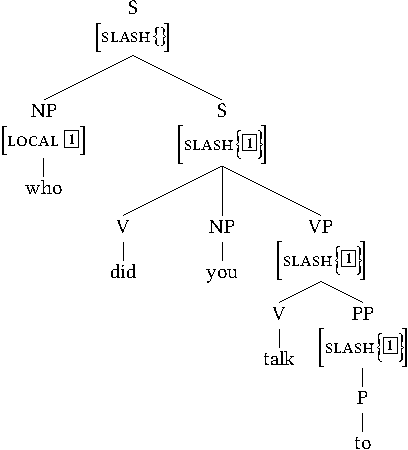
\includegraphics{chapters/BB-udc-basic-tree-crop}

Obviously, we need to ask what ensures that the \textsc{slash} feature plays just
the right role here. First, however, we need to say more about gaps.

On the view of gaps we are focusing on here they are only represented in
\textsc{arg-st} lists. Thus, the preposition \emph{to} in (\ref{ex:UDC:10}) has a gap in its
\textsc{arg-st} list but nothing in its \textsc{comps} list and therefore, no complement
in constituent structure. Gaps have the feature make up given in (\ref{ex:UDC:12}):
\ea
\label{ex:UDC:12}
Representation of gaps:\\
\begin{avm}
    \[local & \@1\\
    nonlocal & \[slash & \{ \@1 \} \] \]
  \end{avm}
\z  


\noindent
Thus, \emph{to} in (\ref{ex:UDC:10}) will have an element of this form in an \textsc{arg-st}
list where \avmbox{1} is NP.

Returning now to \textsc{slash}, a widely assumed approach involves the following
assumptions:

\begin{exe} \ex \begin{xlist} \label{ex:UDC:13}
\ex{The \textsc{slash} value of a head is normally the same as the
  union  of the \textsc{slash} values of its
arguments.}

\ex{The \textsc{slash} value of a phrase is normally the same as that of its head.}
\end{xlist}
\end{exe}

\noindent
We will consider how these ideas are formalized in
Section~\ref{sec:UDC:Middle}. For now we will just discuss their
implications for the analysis of (\ref{ex:UDC:10}).  Essentially they
mean that it has the following more elaborate analysis:

 \begin{figure}[htb]
   \centering
\begin{forest}
sm edges without translation
	[{S[\textsc{slash} \eliste]}
		[{NP[\textsc{local} \ibox{1}]} [what]]
		[{S[\textsc{slash} \sliste{ \ibox{1} }]}
			[{V[\textsc{slash} \sliste{ \ibox{1} }]} [did]]
			[{NP[\textsc{slash} \eliste]} [you]]
			[{VP[\textsc{slash} \sliste{ \ibox{1} }]}
				[{V[\textsc{slash} \sliste{ \ibox{1} }]} [put]]
				[{PP[\textsc{slash} \eliste]} [on the table, roof]]]]]
\end{forest}

%\if0
%    \Tree [ [ what ].{NP\\\begin{avm}
%     \[local \@1 \]
%   \end{avm}} [ [ did ].{V\\\begin{avm}
%     \[slash \{ \@1 \} \]
%   \end{avm}}  [ you ].{NP\\\begin{avm}
%     \[slash \{ \} \]
%   \end{avm}} [ [ put ].{V\\\begin{avm}
%     \[slash \{ \@1 \} \]
%   \end{avm}}  \qroof{on the
% table}.{PP\\\begin{avm}
%     \[slash \{ \} \]
%   \end{avm}}
% ].{VP\\\begin{avm}
%     \[slash \{ \@1 \} \]
%   \end{avm}} ].{S\\\begin{avm}
%     \[slash \{ \@1 \} \]
%   \end{avm}} ].{S\\\begin{avm}
%     \[slash \{ \} \]
%   \end{avm}}
%\fi

\caption{\label{fig:UDC:14}Head-driven \textsc{slash} feature percolation}
   
\end{figure}


\noindent
Clause (\ref{ex:UDC:13}a) is responsible for the \textsc{slash} values
on P and both V's, while clause (\ref{ex:UDC:13}b)
is responsible for the \textsc{slash} values on PP, VP and the lower S. This
approach to the distribution of \textsc{slash} crucially involves heads and is
commonly said to be head-driven.

The lower S in Figure~\ref{fig:UDC:11} and~\ref{fig:UDC:14} is the head of
the higher S, but they do not have the same value for
\textsc{slash}. This is because they represent the top of the
dependency. If information about gaps was available above the top of
the dependency, it would be possible to have another filler higher in
the tree as in (\ref{ex:UDC:15}).

\begin{exe}
  \ex[*]{What do you wonder what Kim saw \gap{}?}   \label{ex:UDC:15}
\end{exe}

\noindent
The top of the dependency in Figures~\ref{fig:UDC:11} and~\ref{fig:UDC:14} is a head-filler-phrase and
the constraint on head-filler phrases needs to ensure that the higher S
is {[}\textsc{slash} \{ \}{]}. One might propose the following constraint:

\ea
%\label{fig:UDC:16}
Head-filler phrase (singleton \textsc{slash} set):\\
   \small\emph{head-filler-ph} $\rightarrow$
  \begin{avm}
   \[slash & \{ \}\\
     hd-dtr & \@1 \[\asort{phrase}
     slash & \{ \@2 \}\]\\
   dtrs & \< \[local & \@2\], \@1\>\]
 \end{avm}
\z

\noindent
This says that a head-filler-phrase is \textsc{slash} \{  \} and has a head
daughter which is a phrase with a single local feature structure in its
\textsc{slash} set and a non-head daughter whose \textsc{local} value is the local feature
structure in the \textsc{slash} set of the head. Standardly, however, a slightly
more general constraint is assumed along the following lines:

\ea
\label{fig:UDC:17}
Head-filler phrase:\\
  \small\emph{head-filler-ph} $\rightarrow$
  \begin{avm}
    \[slash & \@3\\
      hd-dtr & \@1 \[\asort{phrase}
        slash & \{ \@2 \} $~\cup$ \@3 \]\\
      dtrs & \< \[local & \@2\], \@1\>\]
  \end{avm}
\z

\noindent
This allows the \textsc{slash} set of the head to contain more than one member
and any additional members form the \textsc{slash} set of the whole phrase. This
is necessary for an example like (\ref{ex:UDC:18}) from \citet{Chaves:12} where indices
are used to link fillers and gaps.

\begin{exe}
\ex \label{ex:UDC:18}
 This is the person who\emph{\textsubscript{i}} I can't remember
{[}which papers{]}\emph{\textsubscript{j}} I sent copies of \gap{}
\emph{\textsubscript{j}} to \gap{}\emph{\textsubscript{i}}.
\end{exe}

\noindent
Examples of this form often seem unacceptable, but this is probably a
processing matter,  see \citealp{Chaves:12}, section 3 for discussion.
See also Section~\ref{sec:UDC:ResumptivePronouns} for long relativisation with resumption in Hausa or Modern Standard Arabic. 

\section{More on gaps}
\label{sec:UDC:MoreOnGaps}


We now look more closely at the nature of gaps. The central question
here is: what exactly are gaps? We noted in the last section that it
has been widely assumed that gaps are only represented in
\textsc{arg-st} lists but that some HPSG work assumes that they are
empty categories, often called traces. There is a third possibility
which might be considered, namely that gaps are represented in
\textsc{arg-st} lists and in \textsc{valence} lists,
i.e. \textsc{subj} and \textsc{comps} lists, but not in constituent
structures. However, it seems that this position has rarely been
considered. One complicating factor is that there seem to be
differences between complement gaps and both subject and adjunct
gaps. A consequence of this is that the question `what are gaps?'
could have different answers for different sorts of gaps, and in fact
different answers have sometimes been given.

Complement gaps seem to have had rather more attention than subject or
adjunct gaps, perhaps because there are many different kinds of
complements, hence many different kinds of complement gaps. We will look
first at complement gaps, and in particular, the gap in (\ref{ex:UDC:basic}). repeated
here as (\ref{ex:UDC:19}).

\begin{exe}
\ex \label{ex:UDC:19}
What did you put \gap{} on the table?
\end{exe}

\noindent
Probably the most widely assumed position is that gaps are only
represented in \textsc{arg-st} lists
\citep[see][]{Sag:97,Bouma:Malouf:Sag:01,Ginzburg:Sag:01,Sag:10a}. On
this view, the verb \textit{put} will have the
following somewhat simplified structure:

\begin{figure}[htb]
  \centering
\begin{forest}
sm edges without translation
	[{\begin{avm}
	\[\head & \textit{verb} \\
	\textsc{slash} & \sliste{ \ibox{1} } \\
	\textsc{arg-st} & \< NP \[ \textsc{local} & \ibox{1} \\ 
										\textsc{slash} & \sliste{ \ibox{1} }\], PP \> \]
	\end{avm}}
	[put]]
\end{forest}
   \caption{\label{fig:UDC:20}Representation of a slashed preposition (traceless)}
\end{figure}

%\if0
%\Tree  [ put ].{\begin{avm}
	%	\[head & verb\\
	%	slash & \{ \@1 \}\\
	%	\textsc{arg-st} & \< NP \[local & \@1 \\slash & \{ \@1 \}\], PP \>\]
	%\end{avm}
%}
%\fi

\noindent
We ignore the \textsc{comps} feature and the issue of what ensures that the verb
here has the same \textsc{slash} value as the gap. We will discuss the latter in
the next section.

The view that gaps are empty categories was a feature of early HPSG
work, notably \citet{Pollard:Sag:94}, and it has been assumed in some
more recent work e.g. \citet{Levine:Hukari:06,Borsley:09a,Borsley:13,Mueller:14b}. On
this view, the VP will have the following structure:

\begin{figure}[htb]
  \centering
\begin{forest}
sm edges without translation
	[{\begin{avm}
	\[\head & \textit{verb} \\
	\textsc{slash} & \sliste{ \ibox{1} } \]
	\end{avm}}
		[{\begin{avm}
		\[\head & \textit{verb} \\
		\textsc{slash} & \eliste \\
		\textsc{arg-st} & \< \ibox{2} NP, \ibox{3} PP \> \]
		\end{avm}} [put]]
		[{\begin{avm}
		\[\textsc{synsem} & \ibox{2} \[ \textsc{local} & \ibox{1} \\
													\textsc{nonlocal} & \[ \textsc{slash} & \sliste{ \ibox{1} } \] \] \]
		\end{avm}} [$e$]]
		[{\begin{avm}
		\[\textsc{synsem} & \ibox{3} \]
		\end{avm}} [on the table, roof]] ]
\end{forest}
    \caption{\label{fig:UDC:21}Representation of a slashed PP (with trace)}  
\end{figure}

  %% \resizebox{\linewidth}{!}{
%% \Tree [ [ put ].{\begin{avm}
%%     \[head & verb\\
%%       slash & \{ ~ \}\\
%%       arg-st & \< \@2 NP, \@3 PP \>\]
%%   \end{avm}
%% }
%% [ $e$ ].{
%%   \begin{avm}
%%     \[synsem & \@2\[local & \@1 \\nonlocal & \[slash & \{ \@1 \}\]\]\]
%%   \end{avm}
%% }
%% \qroof{on the table}.{
%%   \begin{avm}
%%     \[synsem & \@3\]
%%   \end{avm}
%% } 
%% ].{\begin{avm}
%%     \[head & verb\\
%%       slash & \{ \@1 \}\]
%%   \end{avm}
%% }
%% }

\noindent
Again we ignore the \textsc{comps} feature and how the PP here has the same \textsc{slash}
value as the gap.

It is not easy to choose between these two approaches. One argument in
favour of the first view, advanced, for example, in \citet{Bouma:Malouf:Sag:01}, is that it makes it unsurprising that a gap cannot be one
conjunct of a coordinate structure, as in the following:

\begin{exe} \ex \begin{xlist} \label{ex:UDC:22}
\ex[*]{Which of her books did you find both {[}{[}a review of
\gap{}{]} and \gap{}{]}?}

\ex[*]{Which of her books did you find {[}\gap{} and {[}a review of
\gap{}{]}{]}?}
\end{xlist}
\end{exe}

\noindent
It is not obvious why this should be impossible if gaps are empty
categories.\footnote{Coordination is a problem for any empty category,
  not just the empty categories that represent gaps in some HPSG
  work. Various empty categories have been proposed in the HPSG
  literature, most prominently the empty relativiser of
  \citet{Pollard:Sag:94}. \citet[sec.~15.3.5]{Sag:Wasow:ea:03}
  propose that African American Vernacular English has a
  phonologically empty form of the copula. This analysis requires some
  mechanism to prevent this form from appearing as a conjunct. It is
  likely that a mechanism that can do this will also prevent the empty
  categories that represent gaps from being conjuncts.
  
 }

A second argument in favour of a traceless approach comes from
languages which morphologically treat slashed transitives on a par
with intransitives, like Hausa \citep{crysmann_b04yom} or Mauritian
Creole French \citep{Henri10}. In Hausa and Mauritian, verbs
morphologically register whether a direct object is realised locally
or not: in both languages, a ``short'' form is used with locally
realised direct objects, whereas the long form is used with
intransitives as well as in the case of object extraction.

\begin{exe}

  \ex \gll Sun hūtā̀.\\
  \textsc{3pl.cmpl} rest.\textsc{a}\\
  \glt `They rested.' \label{ex:UDC:Hau:intr}
  \ex \label{ex:UDC:Hau:tr}
  \begin{xlist}
    \ex \gll Sun rāzànā.\\
    \textsc{3pl.cmpl} terrorise.\textsc{a}\\
    \glt `They terrorised (someone).' \hfill \citep[632]{newman_p00}
    \ex \gll Sun rāzànà far̃ar-hū̀lā.\\
    \textsc{3pl.cmpl} terrorise.\textsc{c} civilian(s)\\
    \glt `They terrorised the civilians.' \hfill \citep[632]{newman_p00}
    \ex \gll Far̃ar-hū̀lā nḕ sukà rāzànā.\\
    civilian(s) \textsc{foc} \textsc{3pl.cmpl} terrorise.\textsc{a}\\
    \glt `The civilians, they terrorised.' 
  \end{xlist}
  
\end{exe}

\noindent
Hausa verbs are lexically transitive or intransitive, and they are
classified into one of seven morphological grades.\footnote{We
  restrict discussion here to grade 1, although the syntactic pattern
  is systematic across grades, only giving rise to different patterns
  of exponence. See the Hausa grammars by \citet{newman_p00} and
  \citet{jaggar01:_hausa} for details, and \citet{crysmann_b04yom} for
  evidence in favour of a morphological treatment. } Intransitives
only have a single form (A-form), which is characterised by a long
vowel (in grade 1), cf. (\ref{ex:UDC:Hau:intr}). Transitives, however,
display an alternation depending on the mode of realisation of the
direct object: if used intransitively, they pattern with intransitive
in using the A-form (=long vowel in grade 1), but with an in-situ
direct object (\ref{ex:UDC:Hau:tr}a), they obligatorily surface in the
C-form (\ref{ex:UDC:Hau:tr}b), which has a short vowel in grade
1. Once the direct object is extracted, we find the long vowel A-form
again, in parallel to the intransitive use of transitives and true
intransitives: in sum, the morphology of Hausa treats complement
extraction on a par with argument suppression or lexical
intransitives, i.e. as if the direct object complement simply was not
there. Similar observations appear to hold for Mauritian
\citep{Henri10}. Thus, if nonlocal realisation corresponds to lexical
valence reduction, the Hausa (and Mauritian) facts are
straightforwardly accounted for, whereas the generalisation would be
lost, if gaps were considered phonologically empty syntactic elements.


However, the lexical approach to argument extraction has some possibly
non-trivial implications for other lexical sub-theories of HPSG that
make crucial reference to valence lists, which includes lexical theories of
agreement and case. This is because gaps will not be present on the
valence lists of word-level signs. E.g., the theory of ergativity proposed by \citet{Manning:Sag:99} in terms of
linking patterns between \textsc{arg-st} and valence lists is
actually formulated as constraints on lexemes, since e.g. the linking
of the highest argument to the first element on \textsc{comps}
(=ergative subject) needs to be specified independently of whether
this argument is realised by a local or a non-local dependency. The
same holds of course for the linking of objects in accusative
languages.\footnote{Incidentally, \citet{Crysmann:09} exploits the
  fact that extracted arguments do not appear on the valence lists of
  word-level signs and formulates local case assignment for Nias as a
  constraint on \textit{word}, effectively exempting topicalised
  arguments from objective case assignment. }

Similar considerations apply to agreement: if agreement treats local
and non-local arguments alike, it is clear that agrement controllers
cannot be identified in a general fashion in terms of the valence
features of word-level signs: thus, if agreement relations need make
reference to valence rather than argument structure, this can only be
established at the level of lexemes. The relevant evidence comes from
languages, where the highest argument on \textsc{arg-st} does not
necessarily correspond to the highest grammatical function, i.e
\textsc{subj} valence: while some ergative languages display agreement
with the highest argument on \textsc{arg-st}, like e.g. Udi
\citep{harris_a84udi}, Archi \citep{kibrik94:_archi} shows agreement
with the absolutive argument, suggesting that \textsc{subj} is the
right place to establish the relation
\citep{Crysmann:09}. % \footnote{\citet{Borsley:16:Archi} goes a step
  % further and argues that agreement in this language should be
  % expressed at the level of constituent structure. }
In Nias, we find agreement with \textsc{subj} in the realis, and with
the least oblique argument in the irrealis (\textsc{arg-st}). Finally,
in Welsh, we observe a parallelism in the agreement between subjects
of finite verbs and the objects of prepositions and non-finite verbs:
according to \citet{Borsley89}, a unified treatment can be given if
subjects of finite verbs are the first element on \textsc{comps}, an
assumption that directly captures Welsh VSO word order.\footnote{
  \citet{Borsley:16:Archi} argues on rather different grounds that
  agreement in the Caucasian language Archi involves constraints on
  constituent structure, which will favour a trace-based perspective on
  extraction. }

Given the broad empirical support for valence lists as one of the loci
of case and agreement constraints, it is clear that these constraints
must hold for lexemes, not words under a traceless, lexical
perspective of unbounded dependencies.





% , 
% i.e. \textsc{subj} and \textsc{comps}. They distinguish two notions of
% subject, \textit{a-subject} as the least oblique element on
% \textsc{arg-st} and \textit{s-subject} as the element on the
% \textsc{subj} valence list. While the two notions align in accusative
% languages and for intransitives in ergative languages, they are
% dissociate for transitives in ergative languages. This permits
% generalisation of nominative and absolutive case assigment in terms of
% \textit{s-subject}. If accusative vs.\@ ergative linking is
% independent of extraction --- we have little reason to question this
% in the general case ---, then the relevant generalisations about case
% assignment cannot be stated at the level of \textit{word}. In fact,
% this is why \citet{Manning:Sag:99} explicitly formulate their theory
% of ergativity to the level of \textit{lexeme}.




% According to the theory of
% \citet{Ginzburg:Sag:01}, which is widely adopted, the relationship
% between valence lists (\textsc{subj, comps, spr}) and \textsc{arg-st}
% is constrained by the Argument Realisation Principle, which ensures
% that a \textit{gap} cannot appear on the \textsc{comps} list of
% \textit{word}-level signs, effectively capturing the fact that
% non-local realisation (via \textsc{slash}) entails local
% non-realisation.

% It is clear that theories of case and agreement need to be able to make
% reference to valence lists: \citet{Borsley89} argues convincingly that
% agreement in Welsh is controlled by the first element on
% \textsc{comps}, which corresponds to the object of prepositions or 
% non-finite verbs, as well as the subject of finite verbs, which
% surface immediately to the right of the verb in this VSO
% language. I.e. his proposal that subjects of finite verbs are selected
% via \textsc{comps}     




% Just as case assignment may need to make reference to valence lists,
% so does agreement: for Welsh, \citet{Borsley89} argued that the
% agreement pattern of prepositions and non-finite verbs, which is
% controlled by the post-head complement can be generalised to cover
% subject agreement with finite verbs, once : on the assumption that
% a-subjects are s-subjects of non-finite verbs, yet complements of
% finite verbs and prepositions. In Welsh, prepositions

% Borsley's \citeyear{Borsley89} theory of Welsh
% agreement in terms of agreement with the first element on
% \textsc{comps} can easily be reformulated as a theory of lexemes,
% instead of words. The perspective taken in \citet{Borsley09}, however,
% lends itself more easily  


% However, there are also arguments for the second approach.
% As the following show, gaps generally trigger agreement in the same way
% as overt NPs:

% \begin{exe} \ex \begin{xlist} \label{ex:UDC:23}
% \ex[] {The student knows the answer.}

% \ex[] {The students know the answer.}
% \end{xlist}
% \end{exe}

% \begin{exe} \ex \begin{xlist} \label{ex:UDC:24}
% \ex[]{ Which student do you think \gap{} knows the answer?}

% \ex[]{ Which students do you think \gap{} know the answer?}
% \end{xlist}
% \end{exe}

% \noindent
% If gaps only appear in \textsc{arg-st} lists (of \textit{word}-level
% signs), it
% follows that constraints on agreement must refer to \textsc{arg-st}
% lists. This conclusion seems reasonable in some languages but it looks
% problematic in others. For example, \citet{Borsley09} argues that such
% an approach will miss a generalization in the case of Welsh. In Welsh
% subject-verb agreement is one of a number of cases of agreement
% between a lexical head and an immediately following pronoun. Finite verbs show
% agreement in the form of a suffix with a following pronominal subject,
% as the following illustrate:

% \begin{exe}
%   \ex 
%   \begin{xlist}
%     \ex[]{ \gll Gweles i.\\  see.\textsc{past.1sg}  I\\ \glt ‘I see.’}
%     \ex[]{ \gll Gwelon ni.\\  see.\textsc{past.1pl}
%     we\\ ‘We see.’}
%   \end{xlist}
% \end{exe}

% \noindent
% Non-finite verbs show agreement in the form of a preceding clitic with a following pronominal object, as in the following:

% \begin{exe}
%   \ex
%   \begin{xlist}
%     \ex[]{	\gll Gwnaeth		Emrys 	fy	ngweld	i.\\
%     do.\textsc{past.3sg}	Emrys	\textsc{1sg}	see.\textsc{inf}	I\\
%     \glt ‘Emrys saw me.’}
%     \ex[]{	\gll Gwnaeth		Emrys 	ein	gweld	ni.\\
%     do.\textsc{past.3sg}	Emrys	\textsc{1pl}	see.\textsc{inf}	we\\
%     ‘Emrys saw us.’}
%   \end{xlist}
% \end{exe}

% \noindent
% An approach to Welsh agreement which refers to \textsc{arg-st} lists
% will need to refer to the first member in the case of finite verbs but
% the second member in the case of non-finites. But this misses the fact
% that the agreement is with an immediately following pronoun in both
% cases. Welsh has other cases of agreement. For example, most
% prepositions show agreement in the form of a suffix with a following
% pronominal object, and nouns show agreement in the form of a preceding
% clitic with a following pronominal possessor. In both cases, the
% agreement is with an immediately following pronoun. The facts lead
% \citet{Borsley09} to propose that agreement involves constraints on
% order domains in Welsh. As he shows, this proposal entails that gaps
% must be empty categories in this language.\footnote{\citet{Borsley:16:Archi} argues that an AGR-ST based approach to agreement will also miss a generalization in the case of the Caucasian language Archi and proposes that agreement in this language involves constraints on constituent structure. This also means that gaps must be empty categories.}

% However, this conclusion depends to a very large extent on our
% understanding of where and how agreement relations are established
% (word or lexeme) and how exactly the mapping between \textsc{arg-st}
% and valence lists is established: e.g.\ \citet{Crysmann:09} studies
% agreement in Nias, building on the theory of ergativity of
% \citet{Manning:Sag:99} and suggests that in this language, agreement
% patterns in the realis vs.\ irrealis follow a distinction between
% agreement with a syntactic subject (on \textsc{subj}) and agreement
% with the highest argument (on \textsc{arg-st}). If agreement relations
% may indeed target valence lists, the Welsh data above could just as well
% receive a unified treatment in terms of the first element on
% \textsc{comps}, as suggested previously by \citet{Borsley89}.

% If gaps only appear in \textsc{arg-st} lists, it follows that constraints on
% agreement must refer to \textsc{arg-st} lists. This conclusion seems problematic
% for some languages. Thus, Borsley (2009) argues that agreement involves
% constraints on order domains in Welsh, and \citet{Borsley:16:Archi} argues that
% agreement in the Caucasian language Archi involves constraints on
% constituent structure. If these proposals are sound, gaps must be empty
% categories in these languages.\footnote{Gaps and hence the associated
%   fillers also have case in the same way as overt NPs. If there is any
%   evidence that constraints on case must refer to constituent
%   structures, that will pose a problem for the view that gaps only
%   appear in \textsc{arg-st} lists.}

% \pdfmargincomment{BC: The preceding paragraph is really hard to understand. Without any data, the argument is somehow lost. I suggest either to expand, or to relegate to a footnote.
% }

% \pdfmargincomment[color=red]{BB: It's not really clear to me why. The data is (23) and (24), which show that 'gaps generally trigger agreement in the same way as overt NPs'. If gaps are only represented in \textsc{arg-st} lists, it follows that agreement must be the product of constraints on \textsc{arg-st} lists. Evidence that agreement involves to order domains or constituent structures is problematic for this position and suggests that gaps must be empty categories. Do you think I need to say something about the nature of the evidence?}

\bigskip
We turn now to subject gaps. Here a central question is: how similar or
how different are they to complement gaps? The following illustrate a
well-known contrast, which suggests that they may be significantly
different:

\begin{exe} \ex \begin{xlist} \label{ex:UDC:25}
\ex[]{  Who do you think Kim saw \gap{}?}

\ex[]{ Who do you think \gap{} saw Kim?}
\end{xlist}
\end{exe}

\begin{exe} \ex \begin{xlist} \label{ex:UDC:26}
\ex[]{Who do you think that Kim saw \gap{}?}

\ex[*]{Who do you think that \gap{} saw Kim?}
\end{xlist}
\end{exe}

\noindent
The examples in (\ref{ex:UDC:25}) show that a gap is possible in
object position in a complement clause whether or not it is introduced
by \emph{that}. In contrast, the examples in (\ref{ex:UDC:26}) suggest
that a gap is only possible in subject position in a complement clause
if it is not introduced by \emph{that}. \citet{Pollard:Sag:94}
approach this contrast by stipulating that gaps cannot appear in
subject position. This accounts for the ungrammaticality of examples
like (\ref{ex:UDC:26}b). Examples like (\ref{ex:UDC:26}a) are allowed
by allowing verbs like \textit{think} to take a VP complement and have a
non-empty value for \textsc{slash}. \citet{Ginzburg:Sag:01} offer a very
different account, in which subject gaps appear both in \textsc{arg-st} list
and \textsc{subj} lists. They suggest that examples like (\ref{ex:UDC:26}b) are
ungrammatical because \emph{that} cannot combine with a constituent
which has a non-empty \textsc{subj} list.

An important fact about subject gaps is that they are not completely
impossible in a complement clause introduced by \emph{that}. In
particular, they are acceptable if \emph{that} is followed by an
adverbial constituent. The following illustrates:

\begin{exe}
\ex \label{ex:UDC:27}
Who did you say that tomorrow \gap{} would regret his words?
\end{exe}

\noindent
\citet{Ginzburg:Sag:01} offer an account of such examples, but
\citet{Levine:Hukari:06} argue that it is unsatisfactory. More generally, they
argue that subject gaps are like complement gaps in various respects
and therefore should have the same basic analysis. They propose an
analysis with an empty category for both types of gap. Thus, their
approach differs both from the widely assumed approach, which has no
empty categories, and the approach of Pollard and Sag, which has them
in complement position but not in subject position.

We turn now to adjunct gaps. It is not obvious that there is a gap in
examples like (\ref{ex:UDC:6}) repeated as (\ref{ex:UDC:28}), because
no obligatory constituent is missing.\footnote{This position has initially
  been taken in \citet{Pollard:Sag:94}. } 

\avmoptions{center}
\begin{exe}
\ex \label{ex:UDC:28}
\begin{avm} 
  \{ \normalfont Where\\ \normalfont When\\ \normalfont How\\
  \normalfont Why\}
\end{avm}
did you talk to Lee \gap{}?
\end{exe}

\noindent
However, \cite{hukari.levine:adjunct} show that such examples may display
what are often called extraction path effects , certain phonological or
morphosyntactic phenomena which appear between a gap and the associated
higher structure (see the discussion of example (\ref{ex:UDC:34}) on
page \pageref{ex:UDC:34}). Hence, it seems that they must
involve a filler-gap dependency, on a par with examples with a
complement gap.

Of course there are a variety of positions that are compatible with this
conclusion. \citet{Bouma:Malouf:Sag:01} and \citet[168, fn.~2]{Ginzburg:Sag:01} propose that verbal adjuncts are optional extra complements.
On this view, the gaps in the examples in (\ref{ex:UDC:28}) are complement gaps.
\citet{Levine:03} and \citet{Levine:Hukari:06} argue against this approach
with examples like the following:

\begin{exe}
\ex \label{ex:UDC:29}
In how many seconds flat do you think that {[}Robin found a chair,
sat down, and took off her logging boots{]}?
\end{exe}

\noindent
This is a query about the total time taken by three distinct events.
Levine and Hukari propose that a fairly traditional analysis of verbal
adjuncts in which they are modifiers of VP and combine this with the
assumption that gaps are empty categories. The interpretation of
examples like (\ref{ex:UDC:29}) follows straightforwardly on this
analysis. If indeed argument extraction contrasts with adjunct
extraction in terms of whether the gap is introduced  lexically (on
\textsc{arg-st}) or phrasally, this may
provide a direct account of the fact that the use of a resumptive
strategy in extraction is by and large restricted to arguments. As
discussed by \citet{Crysmann:Reintges:14}, resumptives are obligatory
for arguments in Coptic, whereas gap-type extraction is the only
possibility for modifiers.
 

A rather different approach is developed in \citet{Chaves:09}. Like
\citet{Levine:Hukari:06}, he assumes that verbal adjuncts are
modifiers of VP, but he rejects the idea that gaps are empty
categories. He shows in particular that the possibility for a filler
to correspond to a group is neither limited to adjunct extraction nor
to events, but may also be observed with NP complements whose gaps are
properly contained within each conjunct, as shown by the following
examples: 

\begin{exe} \ex \begin{xlist} \label{ex:UDC:31}
\ex[]{ Setting aside illegal poaching for a moment, how many
sharks\textsubscript{\emph{i} + \emph{j}} do you estimate
{[}{[}\gap{}\emph{\textsubscript{i}} died naturally{]} and
{[}\gap{}\emph{\textsubscript{j}} were killed recreationally{]}{]}?}


\ex[]{ {[}{[}Which pilot{]}\emph{\textsubscript{i}} and {[}which
sailor{]}\emph{\textsubscript{j}}{]} will Joan invite \gap{}
\emph{\textsubscript{i}} and Greta entertain \gap{}
\emph{\textsubscript{j}}
(respectively)?}
\end{xlist}
\end{exe}

% \begin{exe}
%   \ex The [ships$_{x+y}$ that [[a U-boat destroyed \gap{}$_x$ ] and [a
%   kamikaze blew up \gap{}$_y$ ]] were not insured. 
% \end{exe}

\noindent
He suggests that the treatment of coordination must be relaxed in such
a way as to permit the creation of group individuals and group events
on the mother's \textsc{slash} where the daughters' \textsc{slash}
values contain the individual or event variables of the group's
members.  This provides an account of complement extraction as in
(\ref{ex:UDC:31}), but it also provides a
straightforward account of the cumulative scoping facts in
(\ref{ex:UDC:29}).
 

% Instead of a set valued
% \textsc{slash} feature, he has a
% list-valued GAP feature, and he allows words to have modifiers in
% their GAP lists. To accommodate examples like (\ref{ex:UDC:29}) he
% proposes an analysis of coordination which allows structures of the
% following form, where \avmbox{1} combines the properties of \avmbox{2} and
% \avmbox{3}.


% % \pdfmargincomment{BC: The preceding paragraph seems to be lacking crucial information.\textCR 
% %  As far as I remember Chaves relegates the solution to a more sophisticated semantics. 
% %  I am not sure, that we cannot just rename GAP to SLASH. I feel that "combines the properties" should be spelled out. }

% % \pdfmargincomment[color=red]{BB: I'll have to try to figure out how to spell out 'combines the properties".}

% \begin{exe} 
%   \ex \label{ex:UDC:30} 
% %   \pdfmargincomment{BC: Do you really want lists? \textCR
% %   BC: What are the constraints on \avmbox{1}, \avmbox{2}, \avmbox{3} ? \textCR
% %   BC: Why \textsc{gap}?}
  
% %   \pdfmargincomment[color=red]{BB: We can clearly note that it doesn't matter whether the feature is called SLASH or GAP or anything else (maybe by saying 'sometimes called gap' when we first mention SLASH). 

% % I'll have to try to figure out how to spell out 'combines the properties".}
%   \Tree [ {\begin{avm}
%       \[gap & \< \@2 \>\]
%     \end{avm}
%   } {
%     \begin{avm}
%       \[gap & \< \@3 \>\]
%     \end{avm}
%   } ].{
%     \begin{avm}
%       \[gap & \< \@1 \>\]
%     \end{avm}
%   }

% \end{exe}



\section{The middle of the dependency}
\label{sec:UDC:Middle}

In the middle of an unbounded dependency we typically have a phrase
(or a clause) with the same value for \textsc{slash} as a non-head daughter. As
we noted in Section~\ref{sec:UDC:BasicApproach}, it is widely assumed
that this relation is mediated by the head daughter. The \textsc{slash} value
of a head is normally the same as that of its arguments, and the \textsc{slash}
value of a phrase is normally the same as that of its head. However,
as we will see, this head-driven approach to the distribution of \textsc{slash}
hasn't always been adopted.

Central to the head-driven approach is the \textsc{slash} Amalgamation Principle,
which we can formulate as follows, following \citet[199]{Ginzburg:Sag:01}:

\ea
\label{fig:UDC:32}
\textsc{slash} Amalgamation Principle:\\
   \textit{word} $\rightarrow$
   \begin{avm}
     $\slash$\[slash & \@1 $~\cup$ \ldots $~\cup$ \@n\\
       arg-st & \<\[slash & \@1\] ~\ldots~ \[slash & \@n \] \>\]
   \end{avm}
\z

\noindent
This is a default constraint, as indicated by the `$/$'. Essentially,
it says that by default by default the \textsc{slash} value of a word
is the union of the \textsc{slash} values of its arguments.  Being
merely a
default constraint will accommodate examples like the following:

\begin{exe}
\ex \label{ex:UDC:33}
The professor is hard {[}to talk to \gap{}{]}.
\end{exe}

\noindent
Here, the adjective \emph{hard} takes an infinitival complement with a
non-empty \textsc{slash} feature but should not have a non-empty \textsc{slash} feature
itself since the complement is the top of the dependency.\footnote{The
  non-local nature of \textit{tough}-constructions appears to be a
  peculiarity of English: similar constructions in German and French
  do exist, but they feature local (passive-like) dependencies. See
  \citet{abeille_a-godard_d-miller_p-sag_i95} and
  \citet{aguila-multner18} for French, as well as \citet{Mueller:02b}
  for German. Even for English, the unboundedness of the construction
  has been challenged: \citet{Grover:95} questions the acceptability
  of English \textit{tough}-constructions involving a UDC out of
  finite clauses and suggests a local account instead.}

To ensure that the \textsc{slash} value of a phrase is normally the same as that
of its head, much work employs a Slash Inheritance Principle, which
stipulates that a phrase and its head have the same value for \textsc{slash}
except at the top of a dependency (see, e.g. \citealt{Bouma:Malouf:Sag:01}:
20). An alternative approach developed in \citet{Ginzburg:Sag:01} uses
the Generalized Head Feature Principle for this purpose. This says that
a headed-phrase and its head daughter have the same \textsc{synsem} values unless
some other constraint requires something different. Among other things
this ensures that a headed-phrase and its head daughter normally have
the same value for \textsc{slash}.

One argument in favour of a head-driven approach to the distribution
of \textsc{slash} is so-called extraction path effects, certain phonological or
morphosyntactic phenomena which appear between a gap and the
associated higher structure (see \citealt{hukari.levine:adjunct};
\citealt{Bouma:Malouf:Sag:01}:3.2). Irish provides one of many
examples that have been discussed. In Irish, the verbal particle
\emph{goN} only occurs with structures that do not contain gaps, while
\emph{aL} only occurs between a filler and a gap. The following
illustrate:\footnote{In some accounts these particles are taken to be
  complementizers. The N indicates that \emph{go} triggers nasal
  mutation while L indicates that \emph{a} triggers lenition,}

\begin{exe} \ex \begin{xlist} \label{ex:UDC:34}
\ex[]{ \gll Shíl mé goN mbeadh sé ann.\\
thought I \textsc{vpart} would-be he there\\
\glt `I thought that he would be there.'}

\ex[]{ \gll An fear aL shíl mé aL bheadh ann.\\
the man \textsc{vpart} thought I \textsc{vpart} would-be there\\
\glt `the man that I thought would be here'}
\end{xlist}
\end{exe}

\noindent
Within a head-driven approach to \textsc{slash} this is just a contrast between a
verb which is {[}\textsc{slash} \{ \}{]} and a verb which is {[}\textsc{slash}
\{{[} {]}\}{]} and is completely unproblematic.

Early HPSG assumed an approach to \textsc{slash} which was not
head-driven (see \citealt{Pollard:Sag:94}: chapter 4), and related
approaches are assumed in \citet{Levine:Hukari:06} and \citet{Chaves:12}.  A problem
with a head-driven approach is that it says nothing about examples
where an unbounded dependency crosses the boundary of a non-headed
phrase such as a coordinate structure. Thus, it does not deal with
examples of asymmetric coordination like the following:

\begin{exe} \ex \begin{xlist} \label{ex:UDC:35}
\ex[]{ How much can you [drink \gap{}] and [still stay sober]]?}

\ex[]{ How many lakes can we [[destroy \gap{}] and [not arouse public antipathy]]?}
\end{xlist}
\end{exe}
% \pdfmargincomment{BC: Goldsmith (1985) suggests that these are possibly not coordinations. See the discussion in P&S 94} 

% \pdfmargincomment[color=red]{BB: I suspect Chaves argues that they are gaps but I will have to check.}

\noindent
Early HPSG \citep{Pollard:Sag:94} accounts for the distribution of
\textsc{slash} by means of the Nonlocal Feature Principle, and related
principles are proposed by \citet[354]{Levine:Hukari:06} and
\citet{Chaves:12}. These principles ensure that the \textsc{slash}
value of a phrase reflects the \textsc{slash} values of all its
daughters (using set union) and apply equally to headed and non-headed
structures. Thus, the examples in (\ref{ex:UDC:35}) are no problem for
these latter approaches. However, they seem to require some extra element to
handle extraction path effects. So it is not easy to choose between
these approaches and the head-driven approach.

A further point that we should emphasize here is that both approaches to
the distribution of \textsc{slash} allow structures like the following:

\begin{figure}[htb]
  \centering
\begin{forest}
sm edges without translation
	[{[\slasch \sliste{ \ibox{1} } ] }
		[\ldots]
		[{[\slasch \sliste{ \ibox{1} } ] } ]
		[\ldots]
		[{[\slasch \sliste{ \ibox{1} } ] } ]
		[\ldots]]		
\end{forest}
  \caption{\label{fig:UDC:36}Across-the-board (ATB) extraction: conflation of \textsc{slash} values} 
\end{figure}

%% \Tree [ {\ldots{}} {
%%   \begin{avm}
%%     \[slash & \{\@1\}\]
%%   \end{avm}
%% } {\ldots{}} {
%%   \begin{avm}
%%     \[slash & \{\@1\}\]
%%   \end{avm}
%% }
%% {\ldots{}} ].{
%%   \begin{avm}
%%     \[slash & \{\@1\}\]
%%   \end{avm}
%% }

\noindent
In other words, both allow more than one daughter of a phrase with a
non-empty \textsc{slash} value to have the same value. This means that we expect
structures in which a single filler is associated with more than one
gap. Thus, examples like the following are no problem:

\begin{exe} \ex \begin{xlist} \label{ex:UDC:37}
\ex[]{ What did Kim {[}[ cook \gap{} for two hours] and [eat \gap{} in four
minutes]{]}?}

\ex[]{ Which person did you [invite \gap{} [without thinking \gap{} would
actually come]]?}
\end{xlist}
\end{exe}

\noindent
(\ref{ex:UDC:37}a), where the two gaps are in a coordinate structure
is standardly said to be a case of across-the-board
extraction. (\ref{ex:UDC:37}b) is traditionally seen as involving an
ordinary gap followed by a parasitic gap. However, for HPSG all these
gaps have essentially the same status (see \citealt{Levine:Hukari:06}
and \citealt{Chaves:12} for extensive discussion).

\section{The top of the dependency: The diversity of unbounded
dependency constructions}
\label{sec:UDC:Top}

We now look more closely at the top of unbounded dependencies. This is
where diversity of unbounded dependency constructions resides. They are
largely the same at the bottom of the dependency and in the middle, but
at the top of the dependency they differ from each other in a variety of
ways. We noted at the outset that the distinctive higher structure in an
unbounded dependency construction may contain a filler but does not
always. In other words, it may be a head-filler-phrase, but it may not,
and there are a number of other possibilities. Moreover,
head-filler-phrases can have quite different properties in different
constructions.

In the introduction to this chapter we mentioned
\emph{wh}-interrogatives and relative clauses as two examples of
unbounded dependency constructions. In English the former always involve
a head-filler-phrase,\footnote{On some analyses of example like the
  following, \emph{who} is just a subject and not a filler:
\ea
Who knows the answer?
\z
However, for other work this is a filler just like the
  \emph{wh}-elements in the text.} while the later sometimes do but
sometimes don't. There are \emph{wh}-relatives and
non-\emph{wh}-relatives of various kinds. English
\emph{wh}-interrogatives and \emph{wh}-relatives look quite similar.
They seem to involve many of the same lexical items: \emph{who},
\emph{which}, \emph{when}, \emph{where}, \emph{why}, and, as the
following show both may be finite or non-finite:

\begin{exe} \ex \begin{xlist} \label{ex:UDC:38}
\ex[]{  Who should I talk to \gap{}?}

\ex[]{ I wondered {[}who to talk to \gap{}{]}.}
\end{xlist}
\end{exe}

\begin{exe} \ex \begin{xlist} \label{ex:UDC:39}
\ex[]{  someone {[}who I should talk to \gap{}{]}}

\ex[]{ someone {[}to whom to talk \gap{}{]}}
\end{xlist}
\end{exe}

\noindent
But there are differences. \emph{Wh}-interrogatives but not
\emph{wh}-relatives allow \emph{what} and \emph{how}:

\begin{exe} \ex \begin{xlist} \label{ex:UDC:40}
\ex[]{ What did Kim say \gap{}?}

\ex[*]{the thing {[}what Kim said \gap{}{]}}
\end{xlist}
\end{exe}\noindent

\begin{exe} \ex \begin{xlist} \label{ex:UDC:41}
\ex[]{How did Lee do it \gap{} {]}}

\ex[*]{the way {[}how Lee did it \gap{}{]}}
\end{xlist}
\end{exe}

\noindent
In \emph{wh}-interrogatives, \emph{which} combines with a following
nominal except in cases of ellipsis. Thus, in (\ref{ex:UDC:5}), repeated here as (\ref{ex:UDC:42}), \emph{book} is
necessary unless it is clear that books are under discussion.

\begin{exe}
\ex \label{ex:UDC:42}
 Which book did Kim buy \gap{}?
\end{exe}\noindent
Notice also that non-finite \emph{wh}-relatives only allow a PP as a
filler. Thus, (\ref{ex:UDC:43}) is not possible as an alternative to (\ref{ex:UDC:39}c).

\begin{exe}
  \ex[*]{someone {[}who to talk to \gap{}{]}}   \label{ex:UDC:43}
\end{exe}

\noindent
Thus, the fillers in the two constructions differ in a number of ways.
The heads also differ in that \emph{wh}-interrogatives have auxiliary +
subject order in main clauses (unless the \emph{wh}-phrase is the
subject), something which does not occur in \emph{wh}-relatives.

\emph{Wh}-interrogatives and \emph{wh}-relatives are not the only
unbounded dependency constructions that inolve a head-filler phrase.
Topicalization sentences such as the following are another:

\begin{exe} \ex \begin{xlist} \label{ex:UDC:44}
\ex \textsc{Beer} I like \gap{}.
\ex To \textsc{London} I went \gap{}.
\end{xlist}
\end{exe}

\noindent
Unlike \emph{wh}-interrogatives and \emph{wh}-relatives, these are
always finite. Also required to be finite are what have been called
\emph{the}-clauses \citealp{Borsley:04,Sag:10a,Borsley:11}, the components of
comparative correlatives such as (\ref{ex:UDC:45}).

\begin{exe}
\ex \label{ex:UDC:45}
The more I read \gap{}, the more I understand \gap{}.
\end{exe}

\noindent
\emph{The}-clauses have the unusual property that they may contain
the complementizer \emph{that}:

\begin{exe}
\ex \label{ex:UDC:46}
The more that I read \gap{}, the more that I understand \gap{}.
\end{exe}

\noindent
Obviously, this is not possible in \emph{wh}-interrogatives and
\emph{wh}-relatives.

\begin{exe} \ex \begin{xlist} \label{ex:UDC:47}
\ex[*]{I wonder {[}who that Lee saw \gap{}{]}.}

\ex[*]{the man {[}who that Lee saw \gap{}{]}}
\end{xlist}
\end{exe}

\noindent
Within HPSG the obvious approach to the sorts of facts we have just
highlighted involves a number of subtypes of the type
\emph{head-filler-phrase}, as in Figure~\ref{fig:UDC:48}.


\begin{figure}[htb]
  \centering

  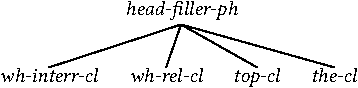
\includegraphics{figures/BB-head-fill-hier-crop}
  \caption{\label{fig:UDC:48}Hierarchy of head-filler phrases}
  
\end{figure}


As was noted in chapter 1, much HPSG work assumes two distinct sets of
phrase types. Assuming this positon, \emph{wh-interr-cl} will not just
be a subtype of \emph{head-filler-ph} but also a subtype of
\emph{interr-cl}, the type \emph{wh-rel-cl} will also be a subtype of
\emph{rel-cl}, and \emph{top-cl} and \emph{the-cl} will both be subtypes
of \emph{decl-cl}. This gives the the type hierarchy in Figur~\ref{fig:UDC:49}

\begin{figure}[htb]
  \centering

  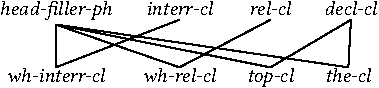
\includegraphics{figures/BB-extraction-function-hier-crop}
  \caption{\label{fig:UDC:49}Hierarchy of extraction clause types (preliminary)}
  
\end{figure}


\noindent
Constraints on \emph{interr-cl} will capture the properties that all
interrogatives share, most obviously interrogative semantics.
Constraints on \emph{rel-cl} will capture what all relatives have in
common, especially modifying an appropriate nominal
constituent.\footnote{Non-restrictive relatives can also modify various
  kinds of non-nominal constituents. See \citet{Arnold:04} and
  \citet{Arnold:Borsley:08}.} Finally, constraints on \emph{decl-cl}
will capture the properties on declaratives, especially declarative
semantics.  Constraints on \emph{wh-interr-cl} and \emph{wh-rel-cl}
will ensure that their fillers take the appropriate form. Constraints
on \emph{top-cl} and \emph{the-cl} will restrict their fillers and
also require their heads to be finite. Further complexity is probably
necessary to handle all the facts noted above. To ensure that
non-finite \emph{wh}-relatives only allow a PP filler while finite
\emph{wh}-relatives allow either an NP or a PP filler it is probably
necessary to postulate two subtypes of \emph{wh-rel-cl}. As for the
fact that \emph{the}-clauses may contain the complementizer
\emph{that}, one way to deal with this is to postulate a subtype of
\emph{head-filler-ph}, \emph{standard-head-fill-ph} with
\emph{wh-interr-cl}, \emph{wh-rel-cl}, and \emph{top-cl} as its
subtypes. This new type will be subject to a constraint preventing its
head from containing a complementizer. The type \emph{the-cl} will not
be a subtype of this new type and hence will be able to contain a
complementizer (see \citealt{Borsley:11} for discussion). All this suggests
the type hierarchy in Figure~\ref{fig:UDC:50}. 
%
\begin{figure}[htb]
  \centering
  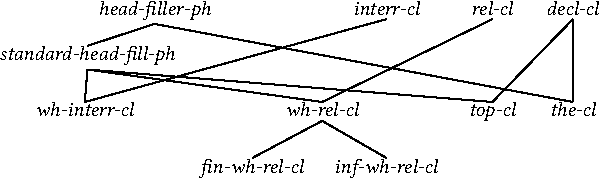
\includegraphics{figures/BB-extraction-function-hier-full-crop}
  \caption{\label{fig:UDC:50}Hierarchy of extraction clause types (final)}
  
\end{figure}
%
%
This is complex, but then the facts are complex, as we have seen.
Crucially, such a hierarchy allows a straightforward account of both the
similarities and the differences among these constructions.

We turn now to cases where there is no filler. We start with the
so-called tough construction, exemplified by (\ref{ex:UDC:33}), repeated here as
(\ref{ex:UDC:51}).

\begin{exe}
\ex \label{ex:UDC:51}
The professor is hard {[}to talk to \gap{}{]}.
\end{exe}

\noindent
Here, there is a gap following the preposition \emph{to}, and the
initial NP \emph{the professor} is understood as the object of
\emph{to}. But this NP is not a filler but a subject. Like any subject
it is preceded by an auxiliary in an interrogative:

\begin{exe}
\ex \label{ex:UDC:52}
 Is the professor hard {[}to talk to \gap{}{]}?
\end{exe}
 
\noindent
Moreover, it is clear that it cannot share a local feature structure
with the gap since it is in a position associated with nominative case
whereas the gap is in a position associated with accusative case. This
suggests that adjectives like \emph{hard} may take an infinitival
complement with a \textsc{slash} value containing a nominal local feature
structure which is coindexed with its subject. The coindexing will
ensure that the subject has the right interpretation without getting
into difficulties over case. It seems, then, that we need something like
the lexical description in (\ref{fig:UDC:53}) in order to account for \emph{hard} in examples like (\ref{ex:UDC:51})
and (\ref{ex:UDC:52}):
  
\ea
\label{fig:UDC:53}
Lexical representation of \textit{tough} adjectives (preliminary):\\
  \begin{avm}
    \[synsem  \[local|cat & \[head & adj\\
          subj & \< NP \[index \@i\] \>\\
          comps & \< VP\[vform & inf\\ slash & \{ NP \[index &
              \@i\] \} \]\>\] \]\]
    \end{avm}
\z

\noindent
But there is more to be said here. \emph{Hard} and its infinitival
complement are the top of a dependency. It is essential that the AP
\emph{hard to talk to} should not have the same \textsc{slash} value as the
infinitival complement \emph{to talk to}. How this should be prevented
depends on what approach is assumed to the distribution of \textsc{slash} values.
However, if this involves a default \textsc{slash} Amalgamation Principle of the
kind discussed in Section~\ref{sec:UDC:Middle}, it is a fairly simple matter. A default
\textsc{slash} Amalgamation Principle ensures that the \textsc{slash} value of a word is
normally the same as the \textsc{slash} value of its arguments. We can override
the principle in the present case by giving adjectives like \emph{hard}
lexical descriptions of the following form:

\ea
\label{fig:UDC:54}
Lexical representation of \textit{tough} adjectives (final):\\*
  \begin{avm}
    \[synsem  \[local|cat & \[head & adj\\
          subj & \< NP \[index \@i\] \>\\
          comps & \< VP\[vform & inf\\ slash & \{ NP \[index &
              \@i\] \} $~\cup$ \@1 \]\>\]\\
        nonlocal & \[slash & \@1 \]
      \]\]
  \end{avm}
\z  

\noindent
This ensures that \textsc{slash} value of such adjectives is the \textsc{slash} value of
the infinitival complement minus the NP that is coindexed with its
subject. Where this NP is the only item in the complement's \textsc{slash} value,
the adjective will be {[}\textsc{slash} \{\}{]}, and so will the AP that it
heads. However, it is possible to have an additional item in the \textsc{slash}
value, as in the following well-known example:

\begin{exe}
\ex \label{ex:UDC:55}
 Which violin is this sonata {[}easy to play \gap{} on \gap{}{]}?
\end{exe}

\noindent
Here, \emph{which violin} is understood as the object of \emph{on} and
\emph{this sonata} as the object of \emph{play}. The infinitival
complement \emph{to play on} will have two items in its \textsc{slash} set, one
associated with \emph{which violin} and one associated with \emph{this
sonata}. The constraint in Figure~\ref{fig:UDC:54} will ensure that only the former appears in the \textsc{slash} set
of \emph{easy} and hence only this appears in the \textsc{slash} set of
\emph{easy to play on}.

The term lexical binding of \textsc{slash} is often applied to situations like
this in which a lexical item makes some structure the top of a
dependency. This is a plausible approach to adjectives like \emph{hard}
and also to adjectives modified by \emph{too} or \emph{enough}, as in the
following:

\begin{exe}
\ex \label{ex:UDC:56}
Lee is too important for you to talk to.
\end{exe}

\begin{exe}
\ex \label{ex:UDC:57}
Lee is important enough for you to talk to.
\end{exe}

\noindent
Lexical binding is also a plausible approach to relative clauses which
have not a filler but a complementizer. This may include English
\emph{that} relatives such as that in (\ref{ex:UDC:58}) (although some HPSG work,
e.g. \citet{Sag:97}, has analysed \emph{that} as a relative pronoun and hence
a filler):

\begin{exe}
\ex \label{ex:UDC:58}
 the man {[}that you talked to \gap{}{]}
\end{exe}

\noindent
If relative \emph{that} is a complementizer, and complementizers, are
heads, as in much HPSG work, it can be given a lexical description
like the one in (\ref{fig:UDC:59}):

\ea
\label{fig:UDC:59}
Lexical representation of relative complementiser \textit{that}:\\*
  \begin{avm}
    \[synsem \[local|cat  \[head & \[{\normalfont\textit{complementizer}}\\ mod 
            \; NP\[index & \@i \]\]\\
          subj & \< \>\\
          comps & \< S\[vform & \normalfont\textit{fin}\\slash & \{ \mbox{\textup{NP}} \[index & \@i \] \} $~\cup$ \@1 \]\> \]\\
      nonlocal  \[slash & \@1 \]\]\]
  \end{avm}
  
\z

\noindent
This says that \emph{that} takes a finite clause as its complement and
modifies an NP, that the \textsc{slash} value of the clause includes an NP which
is coindexed with the antecedent noun selected via \textsc{mod}, and that any additional members of the
complement's \textsc{slash} set form the \textsc{slash} set of \emph{that}. Normally there
will be no other members and \emph{that} will be {[}\textsc{slash}
\{\}{]}.\footnote{This is essentially the approach that is taken to
  relatives in Modern Standard Arabic in \citet{Alqurashi:Borsley:12}.}

Further issues arise with zero relatives, which contain neither a filler
nor a complementizer, such as the following English example:

\begin{exe}
\ex \label{ex:UDC:60}
 the man {[}you talked to \gap{}{]}
\end{exe}

\noindent
For \citet{Sag:97}, these are one type of non-\emph{wh}"=relative and are
required to have a MOD value coindexed with an NP in the \textsc{slash} value of
the head daughter. But an issue arises about semantics. Assuming the
main verb in a zero relative has the same semantic interpretation as
elsewhere, a zero relative will have clausal semantics and not the
modifier semantics that one might think is necessary for a nominal
modifier. Sag's solution is to propose a special subtype of
\emph{head-adjunct-phrase} called \emph{head-relative-phrase}, which
allows a relative clause with clausal semantics to combine with a
nominal and be interpreted in the right way. One might well wonder how
satisfactory this approach is.

\citet{Sag:10a} shows that it is a simple matter to assign modifier semantics
to a relative clause where the basic clause is the daughter of some
other element, as it is when there is a filler or a complementizer. The
basic clause can have clausal semantics and the mother can have modifier
semantics. This suggests that zero relatives too might be analysed as
daughters of another element with modifier semantics. One might do this,
as \citet[531]{Sag:10a} notes, with a special unary branching phrase
type \citep[Section~10.3.2]{Mueller99a}.
Alternatively, one might postulate a phonologically null counterpart of
relative \emph{that}.\footnote{This is the approach that is taken to
  zero relatives in Modern Standard Arabic in \citet{Alqurashi:Borsley:12}.}

There are various other issues about the top of the dependency.
Consider, for example, cleft sentences such as (\ref{ex:UDC:61}).

\begin{exe}
\ex \label{ex:UDC:61}
 It was on the table that he placed the book \gap{}.
\end{exe}

\noindent
Clefts consist of \emph{it}, a form of \emph{be}, a focused constituent,
and a clause with a gap. In (\ref{ex:UDC:61}) the focused constituent is a PP and so
is the gap. It looks, then, as if the focused constituent shares its
main properties with the gap in the way that a filler would. However,
there are also clefts where it is clear that the focused constituent
does not share an index with the gap. Consider e.g. the following:

\begin{exe}
\ex \label{ex:UDC:62}
It's me that \gap{} likes beer.
\end{exe}

\noindent
Here the focused constituent is first person singular, but the gap is
third person singular, as shown by the form of the following verb. Given
the standard assumption that person, number and gender features are a
property of indices, it follows that they cannot have the same index.
There are important challenges here.

Agreement in German may shed some more light on this: 

\begin{exe}
\ex \label{ex:GermanRelAgr}
\begin{xlist}
  \ex[]{\gll Da habe ich,  der/die sonst immer rechtzeitig kommt, doch tatsächlich verschlafen.\\
  there have.\textsc{1sg} I who.\textsc{sg.m}/who.\textsc{sg.f} otherwise always on.time come.\textsc{3sg}, indeed verily overslept\\
  \glt `I,  who is otherwise always on time, have indeed overslept.'} 
  \ex[]{\gll Da habe ich,  der ich sonst immer rechtzeitig komme, doch tatsächlich verschlafen.\\
  there have.\textsc{1sg} I who.\textsc{sg.m} I otherwise always on.time come.\textsc{1sg}, indeed verily overslept\\
  \glt `I,  who is otherwise always on time, have indeed overslept.'}
\end{xlist}
\end{exe}

\noindent 
In (\ref{ex:GermanRelAgr}a), we find a reduced agreement pattern in
number and gender between the relative pronoun and the antecedent
noun, to the exclusion of person. Within the relative clause, however, we find full person/number subject agreement on the verb. In (\ref{ex:GermanRelAgr}b), however, the relative pronoun is post-modified by the pronoun \textit{ich} `I', triggering full  agreement with both the antecedent noun and the embedded verb. 
French, by contrast, observes full agreement of all three \textsc{index} features: 

\begin{exe}
 \ex \label{ex:FrenchRelSAgr} \gll C'est moi qui suis venu(e).\\
  it's me who am come.\textsc{m/f}\\
\glt `It's me who came.' 
\end{exe}
 
\noindent
Thus, relative pronouns and complementisers seem to differ cross-linguistically as to the features which undergo agreement with the antecedent.  

Also quite challenging are free relatives. They look rather like
head-filler-phrases. The initial constituent of a free relative behaves
like a filler, reflecting the properties of the gap.

\begin{exe}
\ex \label{ex:UDC:63}
whichever student you think knows/*know the answer
\end{exe}

\begin{exe}
\ex \label{ex:UDC:64}
whichever students you think know/*knows the answer
\end{exe}

\noindent
But the initial constituent also behaves like a head, determining the
distribution of the free relative.

\begin{exe}
\ex \label{ex:UDC:65}
\begin{xlist}
  \ex[]{Kim will buy what(ever) Lee buys.}
  \ex[*]{Kim will buy where(ever) Lee goes.}
  
\end{xlist}
\end{exe}


\begin{exe}
\ex \label{ex:UDC:66}
\begin{xlist}
  \ex[]{Kim will go where(ever) Lee goes.}
  \ex[*]{Kim will go what(ever) Lee buys.}
\end{xlist}
\end{exe}

\noindent
In case languages like German, the matching effect generally includes case
specifications \citep{Mueller:99a}. % In order to reconcile 
% mismatches between the case requirement that is internal to the relative
% clause and the one that is selected for the free relative as whole,
% \citet{Mueller:99a} suggests a unary schema that mediates between the
% different case requirements.  

Most work on free relatives has
assumed that it is a filler and not a head
\citep{Groos:Riemsdijk:81,Grosu:2003} or a head and not a filler
\citep{Bresnan:Grimshaw:78}. But the obvious suggestion is that it is
both a filler and a head, a position espoused in
\citet{Huddleston02}. This idea can be implemented within HPSG by
analysing free relatives and head-filler-phrases as subtypes of
filler-phrase, as follows:


\begin{figure}[htb]
  \centering

  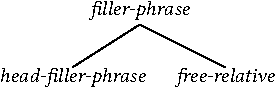
\includegraphics{figures/BB-filler-phrase-crop}
  \caption{\label{fig:UDC:67}Hierarchy of filler phrases}
  
\end{figure}

\noindent
Filler-phrase will be subject to a constraint like that proposed earlier
for head-filler-phrases except that it will say nothing about the
head-daughter. Head-filler-phrases will be subject to a constraint
identifying the second daughter as the head, while free-relatives will
be subject to a constraint identifying the first daughter as the head
(among other things).\footnote{The constraint on free relatives will also
  need to ensure that the first daughter takes the appropriate form and
  that the second daughter is finite.}

Naturally, there may be complications here. German, for example, has
some free relatives in which the case of the \emph{wh}"=element differs from
that which the position of the free relative leads one to expect. This
looks like a problem for the idea that the initial constituent is a
head, but it may not be if heads and the associated phrases only share
syntactic properties by default, as in much HPSG
work.\footnote{\citet{Mueller:99a} pursues a rather different approach
  to free relatives: In order to reconcile 
mismatches between the case requirement that is internal to the relative
clause and the one that is selected for the free relative as whole,
he suggests a unary schema that mediates between the
different case requirements.  }


\section{Resumptive pronouns}
\label{sec:UDC:ResumptivePronouns}

Ever since \citet{Vaillette:01}, resumption has been treated as an unbounded dependency within HPSG, on a par with \textsc{slash} dependencies, rather than as a case of anaphoric binding. The main motivation for treating resumption similar to extraction lies with the fact that in a variety of languages dependencies involving a pronominal at the bottom of the dependency behave similarly to UDCs involving a gap at the extraction site. 

\citet{Vaillette:01} investigates resumption in Hebrew and shows on
the basis of across-the-board (ATB) extraction, parasitic gaps, and
crossover that resumptive dependencies are indistinguishable from gap
dependencies except for their reduced sensitivity to extraction
islands. In order to reconcile the UDC-like properties of resumption
with the difference in island sensitivity, he introduces a dedicated
non-local feature \textsc{resump}. While using separate features for
resumptives and gaps easily makes them distinguishable for the
purposes of island constraints, it certainly has the drawback that
formulation of the ATB constraint becomes quite cumbersome.
The following example illustrates mixing of gaps and resumptives in
ATB extraction in Hebrew: 

\begin{exe}
  \ex \label{ex:HebATB}{\gll kol
profesor$_i$ še dani roce lehazmin \gap{}$_i$ aval lo maarix \textbf{ʔoto}$_i$ maspik
\\
every professor that Dani wants to-invite {} but not
esteems him enough\\
\glt `every professor that Dani wants to invite but doesn’t respect
enough'\hfill\citep[78]{sells_p84}}
\end{exe}

\noindent
Subsequent work on Persian \citep{taghvaipour:phd:05}, Welsh
\citep{Borsley:13} and Hausa \citep{Crysmann:12} essentially follows
Vaillette, using ATB extraction as the main indicator for treating
resumptive dependencies similar to gap dependencies. What all these
works have in common, though, is that they rely on a single non-local
feature, namely \textsc{slash} for both types of dependencies. In
particular these works suggest that mixing of strategies, as
illustrated in (\ref{ex:HebATB}) for Hebrew and in (\ref{ex:HauATB})
for Hausa, suggests that both extraction
strategies should be captured using a single non-local feature,
i.e. \textsc{slash}. Despite this commonality, however, approaches
differ as to how gap and resumptive dependencies are distinguished, if
at all.

In his work on Welsh unbounded dependencies, \citet{Borsley:10}
observes that the choice between gap and resumptive is essentially
determined by properties of the immediate environment of bottom of the
dependency: i.e. while possessors of nouns and complements of
prepositions require a resumptive element when extracted, subjects, as
well as direct objects of finite and non-finite verbs only extract by
means of filler-gap dependencies. Thus, the distribution of gaps vs.\
resumptives is practically disjoint.

Furthermore, he reports evidence that resumptives and gaps also
pattern alike with respect to island constraints: while extraction out
of the clausal complement in a complex NP is fine, with either a gap
or a resumptive at the bottom, extraction out of a relative leads to
ungrammaticality, again, independent of whether we find a gap or a
resumptive.

% Cite ex. (44) and (45)
\begin{exe}
  \ex[]{\gll Dyma ’r dyn y credodd
Dafydd [y si
[y gwelodd
Mair (o)]].\\
here-is the man PRT believe.PAST.3S Dafydd \spacebr{}the rumour \spacebr{}PRT see.PAST.3S Mair he\\
\glt `Here’s the man who David believed the rumour that Mair saw.'}
  \ex[]{ \gll Dyma ’r dyn y credodd Dafydd [y si [y cest ti ’r llythyr ’na ganddo (fo)]].\\
    here-is the man PRT believe.PAST.3SG Dafydd \spacebr{}the rumour \spacebr{}PRT get.PAST.2SG you the letter DEM with.3S.M him\\
    \glt`‘Here’s the man who David believed the rumour that you got that letter
from.'}
    \ex[*]{ \gll Dyma ’r ffenest darais i [’r bachgen [dorrodd (hi) ddoe]].\\
    that-is the window hit.PAST.1S I \spacebr{}the boy \spacebr{}break.PAST.3S (she) yesterday\\
    \glt
    }
\end{exe}

\noindent
Moreover, with respect to the across-the-board (ATB) constraint resumptives and gaps show
the same behaviour as observed for Hebrew, easily permitting
mixing. In addition, Welsh also has certain extraction path effects which are the same in gap and resumptive dependencies  \citep[see][for details]{Borsley:10}. 

Given that the distribution of gaps and resumptives is regulated by the locally selecting head at the bottom of the dependency and that there is no need to distinguish the two types of dependencies along the extraction path (middle), \citet{Borsley:10} formulates what is probably the most simple and straightforward approach to resumption. In essence, he proposes``that we need
structures in which a slashed preposition or noun has not a slashed argument
but a pronominal argument coindexed with its slashed
value''. Consequently he extends \textsc{Slash Amalgamation} to
optionally include a \textsc{slash} element coindexed with an
unslashed pronominal argument. This move licenses Welsh resumptives in
a structure like the one in Figure~\ref{fig:WelshResump} below:  

\begin{figure}[htb]
  \centering
\begin{forest}
sm edges without translation
	[{\begin{avm}
			\[\head & \ibox{1} prep $\vee$ noun \\
			\textsc{slash} & \sliste{ \ibox{2} NP$_i$ } \]
	\end{avm}}
	[{\begin{avm}
			\[\head & \ibox{1} \\
			\textsc{slash} & \sliste{ \ibox{2} } \\
			\textsc{arg-st} & \sliste{ \ldots{} \ibox{3} \ldots{} } \]
	\end{avm}}]
	[{\ibox{3} NP$_i$ }]
	[\dots]]
\end{forest}
    \caption{\label{fig:WelshResump}Representation of Welsh resumptives}  
\end{figure}


%%     \Tree [ 
%% {
%%     \begin{avm}
%%         \[head & \@1 \\
%%         slash & \{ \@2 \} \\
%%         arg-st & \< ... \@3 ... \> \]
%%     \end{avm}
%%   }
%%   { \avmbox{3}NP$_i$ } { ... }  
%% ].{
%%     \begin{avm}
%%         \[head & \@1 prep $\vee$ noun\\
%%         slash & \{ \@2 NP$_i$ \} \]
%%     \end{avm}
%%     }
\noindent
Thus, the only difference between gaps and resumptives on his account
is that the former give rise to a reentrancy of an element in
\textsc{slash} with a \textsc{local} value on \textsc{arg-st}, whereas the latter merely involve reentrancy of \textsc{index} values (between an NP \textit{local}  on \textsc{slash} and an NP \textit{synsem} on \textsc{arg-st}).  

The respective distribution of gaps and resumptives are finally
accounted for by means of constraints on the binding theoretical
status of the element at the bottom of the the dependency,
i.e. \textit{ppro} for resumptives and \textit{npro} for gaps.

Borsley's decision to locate the resumptive function on the selecting head, rather than on the pronominal not only provides a good match for the Welsh data, but it also addresses McCloskey's generalisation \citep{mccloskey02:_resum_succes_cyclic_local_operat} that resumptives are always the ordinary pronouns, since no lexical ambiguity between slashed and unslashed pronouns is involved here.  

In contrast to Borsley, who developed his theory of resumption on the
basis of a language where the distribution of gaps vs.\ resumptives is
entirely regulated by the immediate local environment and no difference in island sensitivity could be observed, \citet{Crysmann:12} developed an alternative account for Hausa, a language where the distributions of gaps and resumptives partially overlap at the bottom of the dependency and where resumptive dependencies observe different locality constraints when compared to filler-gap dependencies. 

Hausa patterns with a number of resumptive languages, including Welsh, in that use of a resumptive is obligatory for complements of a preposition or the possessor of a noun. With direct and indirect objects, however, both resumptives and gaps are possible: 

\begin{exe}
  \ex \label{ex:HauIO}
  \begin{xlist}
    \ex{\gll mutā̀nên dà sukà ƙi sayar wà \gap{} dà àbinci
      sukà fìta\\
      men \textsc{rel} \textsc{3.p.cpl} refuse sell to {} with food \textsc{3.p.cpl} left\\
      \glt `the men they refused to sell food to left.' \hfill
      \citep{jaggar01:_hausa}} \ex{\gll mutā̀nên dà sukà ƙi sayar \textbf{musù}
      dà àbinci
      sukà fìta\\
      men \textsc{rel} \textsc{3.p.cpl} refuse sell to.them with food \textsc{3.p.cpl} left\\
      \glt `the men they refused to sell food to left.' \hfill
      \citep{jaggar01:_hausa}}
  \end{xlist}
\end{exe}


\noindent
In (\ref{ex:HauIO}), both a bare dative marker \textit{wà} `to' is possible (with a gap), and a dative pronoun \textit{musù} `to.them'.

Moreover, gap and resumptive dependencies do behave differently with respect to strong islands: while extraction out of a relative clause or \emph{wh}"=island is impossible for gap dependencies, relativisation out of these islands is perfectly fine with resumptives. 

\begin{exe}
  \ex{\gll Gā̀ tābōbîn$_j$ dà
    Àli ya san mùtumìn$_i$ dà
    zâi$_i$ yī \textbf{musù}$_j$ / *{wà \gap{}$_j$}   kwālī\\
    here.is cigarettes \textsc{rel} Ali \textsc{3.s.m.cpl} know man
    \textsc{rel} \textsc{3.s.m.fut} do to.them / to {}   box\\
    \glt `Here are the cigarettes that Ali knows the man that (he) will
    make a box for.' \hfill \citep{tuller_l86} } \label{ex:HauResLongIO}
\end{exe}

\noindent
Crysmann further emphasises that relativisation (which may escape
strong islands) resembles anaphoric relations, whereas filler-gap
dependencies, as observed with \emph{wh}"=fronting, give rise to a matching
effect. He therefore correlates relative complementisers and
resumptives with minimal \textsc{index} sharing, whereas filler-head
structures, as well as gaps will require sharing of entire
\textsc{local} values: while filler-head structures impose this
stricter constraint at the top of the dependency, gaps obviously do so
at the bottom. In order to express constraints on locality,
\citet{Crysmann:12} proposes that \textsc{slash} elements (of type
\textit{local}) should be distinguished as to their weight: while the
type \textit{local} always minimally includes indexical information,
its subtypes \textit{full-local} and \textit{weak-local} differ as to
the amount of additional information that must or must not be
present. For \textit{full-local}, which is appropriate for
\textit{synsem}, this includes categorial and full semantic
information, whereas exactly this information is excluded for
\textit{weak-local}.



\begin{figure}[htb]
  \centering
  
  \begin{tabular}{cc}
    \multicolumn{2}{c}{
    \rnode{l}{\begin{avm}
      \[\asort{local} 
      cont & \[index & ind \]\]
    \end{avm}}
}\\[4em]
    \rnode{f}{\begin{avm}
      \[\asort{full-local}
        cat & cat\\
      \]
    \end{avm}}
    &
      \rnode{w}{\begin{avm}
      \[\asort{weak-local}
        cont & \[rels \< ~ \>\]
      \]
    \end{avm}}
  \end{tabular}
  \psset{angleA=-90,angleB=90,nodesep=1pt,arm=0pt,linewidth=.5pt}
  \ncdiag{l}{w}
  \ncdiag{l}{f}

  
  
  \caption{\label{fig:local}Hierarchy of \textit{local} \citep{Crysmann:12}}
  
\end{figure}

\begin{figure}[htb]
  \centering
\begin{forest}
sm edges without translation
[{\begin{avm}
	\[\asort{synsem}
	loc & full-local \\
	nloc & non-local\]
\end{avm}}
	[{\begin{avm}
	\[\asort{slashed}
	loc & \[\cont|index & \ibox{1} \] \\
	nloc & \[sl & \sliste{ \[cont|index & \ibox{1} \] } \] \]
	\end{avm}}
		[{\begin{avm}
		\[\asort{gap}
		loc & \ibox{1} full-local \\
		nloc & \[sl & \sliste{ \ibox{1} }\] \]
		\end{avm}} ]
		[\textit{resump}]]]
\end{forest}
  \caption{\label{fig:synsem}Hierarchy of \textit{synsem} objects \citep{Crysmann:12}}
\end{figure}

%%     \begin{tree}
%%     \psset{treesep=24ex,levelsep=10ex, linewidth=.5pt}
%%     \br{
%%       \begin{avm}
%%         \[\asort{synsem}
%%         loc & full-local\\
%%         nloc & non-local\]
%%       \end{avm}
%%     }{
%%       \avmoptions{top} \psset{treesep=24ex,levelsep=24ex} \br{
%%         \begin{avm}
%%           \[\asort{slashed}
%%           loc & \[cont|index & \@1\]\\
%%           nloc & \[sl \{ \[cont|index & \@1\] \}\]\]
%%         \end{avm}
%%       }{\psset{linestyle=solid} \lf{
%%           \begin{avm}
%%             \[\asort{gap}
%%           loc & \@1 full-local\\
%%           nloc & \[sl & \{ \@1 \}\]\]
%%         \end{avm}
%%       } \lf{\textit{resump}
%%       } }}
%% \end{tree}

The hierarchy of \textit{local} types provides for the possibility
that \textit{local} types on \textsc{slash} may only be partially
specified: while gaps and filler-head structure require full
reentrancy of a (\textit{full-local}) \textsc{local} value,
resumptives may be non"=committal with respect to the weight
distinction, only imposing the minimal index-sharing constraint. This
ensures that both resumptives and gaps can be found at the bottom of a
strong UDC with e.g.\ a \emph{wh}"=filler. Conversely, islands can narrow down
the nature of \textsc{slash} elements to only pass on a \textsc{slash}
set of \textit{weak-local}, such that resumptives, but not gaps will
be licensed at the bottom in the case of long relativisation.

Underspecification of \textit{local} at the bottom of a resumptive
dependency easily permits mixing of gap and
resumptive strategies in ATB extraction, as illustrated by the example
below:

  \begin{exe}
  \ex{\gll [àbōkī-n-ā]{$_i$} dà [[na zìyartā̀ \gap{}$_i$] àmmā [bàn sā̀mē \textbf{shì}$_i$ à gidā
    ba]]\\
    \spacebr{}friend-\textsc{l-1.s.gen} \textsc{rel} \hspaceThis{[[}\textsc{1.s.cpl} visit {} but
    \spacebr{}\textsc{1.s.neg.cpl} find \textsc{3.s.m.do} at home \textsc{neg}
    \\
    \glt `my friend that I visited but did not find at home' \hfill \citep[539]{newman_p00}
   }    \label{ex:HauATB}

\end{exe}

The obvious question is of course how these two approaches can be harmonised in order to yield a unified HPSG theory of resumption.  It is clear that the theory advanced by \citet{Crysmann:12} makes a more fine-grained distinction with regard to \textsc{slash} elements and should therefore be able to trivially account for languages where there is no difference in locality restrictions between resumptive and gap dependencies. In the case of Welsh, it will suffice to strengthen the constraints of strong islands, such as relative clauses to block passing of any \textit{local} on \textsc{slash}, rather than merely restricting to \textit{weak-local}. The other area where the theories need to be brought closer together concerns the issue of McCloskey's generalisation, which is straighforwardly derived by a syntactic theory of resumption, such as Borsley's. Some work in this direction has already been done: \citet{Crysmann:16} suggests  replacing his original ambiguity approach with an underspecification approach, essentially following \citet{Borsley:10} in locating the disambiguation between pronoun and resumptive function on the selecting head. While there are still differences of implementation, general agreement has been obtained that it should indeed be the head that decides on the pronominal's function, whether this is done via disjunctively amalgamating the index of a pronominal argument  \citep{Borsley:10,Alotaibi:Borsley:13}, or else via a more elaborate system of \textit{synsem} types that integrates more nicely with standard \textsc{slash} amalgamation \citep{Crysmann:16}. 

Similar consensus has been reached with respect to the need to have more fine-grained control on locality, again irrespective of implementation details: while \citet{Alotaibi:Borsley:13} exploited constraints on case marking in order to capture the difference in locality of  resumptives and gaps in Modern Standard Arabic, the weight-based analysis by  \citet{Crysmann:17} provides a more principled account of the data, essentially obviating stipulative nominative case assignment that fails to correspond to any overtly observable case marking.  

Some questions still remain: \citet{taghvaipour:phd:05} claims that in
Persian, the distribution of gaps vs.\ resumptives is partly
determined by the constructional properties of the top of the
dependency, showing different patterns for non-restrictive,
restrictive and free relative clauses, and suggests that
constructional properties of the top need to be transmitted via
\textsc{slash}.  However, percolation of constructional information
across the tree appears to does not play nicely with basic assumptions
of locality within HPSG. It remains to be seen how the case of Persian
can be analysed within the scope of the theories outlined above. 

Another case study that deserves integration into the current HPSG theory of resumption concerns so-called hybrid chains in Irish \citep{assmann10:_does_chain_hybrid_irish_suppor}: in this language,  the most deeply embedded complementisers register the difference between gaps and resumptives at the bottom, yet complementisers further up can switch between ``resumptive marking'' and ``gap marking''. While the authors use a single \textsc{slash} feature for both types of dependency, the objects on this set remain incompatible, thereby necessitating a great deal of disjunction. In order to bring this analysis fully in line with current HPSG,  underspecification techniques may be fruitfully explored.  


%\begin{itemize}
%\item Evidence for a \textsc{slash} analysis %\citep{Vaillette:01,Vaillette:02,taghvaipour:phd:05,Borsley:10,Borsley:13,Crysmann:12,Crysmann:16,Crysmann:17} 
%\item The nature of resumptive pronouns \citep{Borsley:10,Alotaibi:Borsley:13,Crysmann:12,Crysmann:16,Crysmann:17} 
%\end{itemize}

\section{More on \emph{wh}"=interrogatives}
\label{sec:UDC:MoreWh}

\subsection{Pied piping}

So far, we have concentrated on unbounded dependencies as witnessed by extraction, captured in HPSG by \textsc{slash} feature inheritance. Another type of unbounded dependency is featured by pied-piping, as illustrated in (\ref{ex:WhPiedPiping}) and (\ref{ex:RelPiedPiping}), taken from \citet{Ginzburg:Sag:01}. 

\begin{exe}
  \ex \label{ex:WhPiedPiping}
  \begin{xlist}
    \ex{I wonder [[\textit{what}] inspired them]. }
    \ex{I wonder [[\textit{whose} cousin] ate the pastry].} 
    \ex{I wonder [[\textit{whose} cousin's dog] ate the pastry].} 
    \ex{I wonder [[to \textit{whom}] they dedicated the building]}
  \end{xlist}
\end{exe}

\begin{exe}
  \ex \label{ex:RelPiedPiping}
  \begin{xlist}
    \ex{the book [[\textit{which}] inspired them] }
    \ex{the person [[\textit{whose} cousin] ate the pastry]} 
    \ex{the person [[\textit{whose} cousin's dog] ate the pastry]} 
    \ex{the person [[to \textit{whom}] they dedicated the building]}
  \end{xlist}
\end{exe}

\noindent
In (\ref{ex:WhPiedPiping}) the \emph{wh}"=word, a pronoun or determiner, that
marks the (embedded) \emph{wh}"=interrogative clause may be arbitrarily deeply embedded inside the filler.  

With relative clauses, as witnessed by (\ref{ex:RelPiedPiping}), the relative pronoun may be embedded inside the filler, and, again, arbitrarily deep. Furthermore, regardless of the level of embedding,  the relative pronoun is coreferent with the antecedent noun, such that a mechanism is called for that can establish this token identity in a non-local fashion. This is most evident in languages where relative undergo agreement with the antecedent noun, as e.g. in German: 

\begin{exe}
\ex
  \begin{xlist}
    \ex{\gll das Buch [\textit{das} mich inspirierte]\\
        \textsc{def.n.s} book(\textsc{n})\textsc{.s} \hspaceThis{[}\textsc{rel.n.s} me inspired\\
        \glt `the book that inspired me'
        }
    \ex{\gll die Person [\textit{die} mich inspirierte]\\
        \textsc{def.f.s} person(\textsc{f})\textsc{.s} \hspaceThis{[}\textsc{rel.f.s} me inspired\\   
        \glt `the person that inspired me'}
    \ex{\gll das Buch [[\textit{dessen/*deren} Einband] mir gefiel ]\\
        \textsc{def.n.s} book(\textsc{n})\textsc{.s} \hspaceThis{[[}\textsc{rel.n.s.poss} cover me pleased\\
        \glt `the book the cover of which I like'}
    \ex{\gll die Autorin [[\textit{deren/*dessen} Roman] mir gefiel ]\\
            \textsc{def.f.s} author(\textsc{f})\textsc{.s} \hspaceThis{[[}\textsc{rel.f.s.poss} novel me pleased\\
        \glt `the (female) author whose novel I liked'}
  \end{xlist}
\end{exe}

\noindent
In order to capture  the fact that the filler of a \emph{wh}"=clause must
contain a \emph{wh}"=word, or that the relative pronoun contained within the
filler of a relative must be structure-share its \textsc{index} with the antecedent noun, HPSG builds on previous work in GPSG \citep{Gazdar85}, postulating the non-local features \textsc{que/wh} and \textsc{rel}. \citet{Pollard:Sag:94} have proposed a single \textsc{Nonlocal} Feature Principle that generalises from \textsc{slash} feature percolation to inheritance of \textsc{que} and \textsc{rel}, defining the value of each non-local feature of the mother as the set union of the nonlocal features of the daughters. See, however, \citet{Sag:97} and \citet{Ginzburg:Sag:01} for head-driven formulation of nonlocal feature percolation. 

One observation regarding pied piping in languages such as English or German pertains to the fact that \emph{wh}"=words tend to surface in the left periphery of the filler. \citet{Ginzburg:Sag:01} suggest that amalgamation of \textsc{que/wh} is restricted to the least oblique element on \textsc{arg-st}. This enables them to rule out  (\ref{ex:WhPiedPipingOblique}b) while still being able to account for standard pied-piping with prepositional phrases (\ref{ex:WhPiedPiping}d). 

\begin{exe}
  \ex \label{ex:WhPiedPipingOblique}
  \begin{xlist}
  \ex[]{ I wonder [[whose picture] was on display].}
  \ex[*]{I wonder [[my picture of whom] was on display].}
  \end{xlist}
\end{exe}

\noindent
Indeed, from a cross-linguistic perspective, pied-piping of prepositions appears to be the far less marked option when compared to preposition stranding, which appears to be a peculiarity of English. This is supported not only by the ban on preposition stranding in German and many other languages (or its restriction to \textit{avec/sans} `with'/`without' in French),  but it is also corroborated by the distribution of resumptives (see section \ref{sec:UDC:ResumptivePronouns}). 

To summarise, pied piping in HPSG is understood as a phenomenon that involves a second unbounded dependency: in addition to a \textsc{slash} dependency between the pied-piped filler and the extraction site, just like the ones we have discussed throughout this chapter, \textsc{que} or \textsc{rel} establish dependencies within the filler itself. 

\subsection{Multiple \emph{wh}"=questions}

% G&S on English

While in languages such as English only one \emph{wh}"=phrase may be fronted per interrogative clause (and typically one phrase is indeed fronted), it is nevertheless possible to ask multiple questions, with additional \emph{wh}"=phrases remaining in situ, as witnessed by \textit{what} in (\ref{ex:WhMult}).  

\begin{exe}
  \ex Who asked who saw what? \label{ex:WhMult}
\end{exe}

\noindent
According to the theory of \citet{Ginzburg:Sag:01}, only fillers in interrogative clauses are \emph{wh}"=marked, and \emph{wh}"=marking serves to ensure that a \emph{wh}"=quantifier contained in the filler is interpreted as a parameter of the local interrogative clause. In situ \emph{wh}"=phrases,  by contrast, are still quantifiers, so they may scope higher than their syntactic position suggests. 
\citet{Ginzburg:Sag:01} follow \citet{Pollard:Sag:94} in adopting a
Cooper storage, which enables them to have the in situ \emph{wh}"=quantifier
in (\ref{ex:WhMult}) retrieved either as a parameter of the embedded
interrogative clause, or as a parameter of the matrix question. The
\textsc{wh}  feature thus not only ensures that a \emph{wh}"=interrogative is
marked as such by a filler containing a \emph{wh}"=word, but it also fixes the
semantic scope of ex-situ % \pdfcomment{BC: The term is quite frequently
  % used in the focus literature. }
\emph{wh}"=phrases to their syntactic
scope.\footnote{\citet{kathol:scope-marking} uses the \textsc{que}
  feature in his analysis of partial \emph{wh}"=fronting in German. } In situ \emph{wh}"=quantifiers, by contrast, are permitted to take arbitrarily wide scope. 

In Slavic languages such as Russian or Serbo-Croatian \citep{Penn:99},
there does not appear to be a constraint on the number of simultaneously fronted \emph{wh}"=phrases, as illustrated by the example in (\ref{ex:WhMultFront}). 

\begin{exe}
  \ex \label{ex:WhMultFront}
  \begin{xlist}
  \ex[]{\gll Ko koga si mislio da je voleo?\\
  who whom \textsc{CL-2s} thought Comp \textsc{CL-3s} loved\\
  \glt `Who did you think loved whom?' \citep{Penn:99}}
 
  \ex[*]{Ko si koga mislio da je voleo?}
  \end{xlist}
\end{exe}

\noindent
Given that HPSG's nonlocal features, and in particular \textsc{slash}
and \textsc{que/wh}, are set valued, multiple \emph{wh}"=fronting is a rather
expected property. In fact, the grammar of English interrogatives as
proposed by \citet{Ginzburg:Sag:01} specifically stipulates that there
be only a singleton \textsc{wh} set, and that head-filler structures
cannot be recursive.
% \pdfcomment{BC: ``Under those circumstances, what
%   shalll we do?' may have two \textsc{slash} elements, but only a
%   single \textsc{wh} element, no?}  

The point where Slavic multiple fronting poses a challenge is its interaction with second position clitics:  it seems, as witnessed by the contrast in (\ref{ex:WhMultFront}) that multiple fronted \emph{wh}"=phrases are treated as a constituent, as far as linearisation is concerned. \citet{Penn:99} proposes a topological analysis based on extended word order domains \citep{Reape:90,kathol_a00} in order to reconcile multiple fronted constituents with the second position property: in essence, 
multiple fillers are assigned to the same initial topological field and linearisation of clitics proceeds relative to that same initial field.   

% Multiple ex-situ wh 

\subsection{\emph{Wh}-in-situ}
\label{sec:UDC:WhInSitu}

In the previous subsections, as in most of this chapter, we have capitalised on ex situ \emph{wh}"=constructions. However, even in languages like English, and even more in French, we do find constructions with clear interrogative semantics where nonetheless the \emph{wh}"=phrase stays in situ. Moreover, in languages such as Japanese or Coptic Egyptian in situ realisation is the norm, rather than the exception. In this subsection we shall therefore discuss how HPSG's theory of unbounded dependencies has been put to use to account for this phenomenon. 

In languages such as English, where  standard \emph{wh}"=interrogatives are signalled by a \emph{wh}"=phrase ex situ (i.e. by a \emph{wh}"=filler),   
\citet{Ginzburg:Sag:01} identify two types of in situ \emph{wh}"=questions in English: so called reprise (or ``echo'') questions, which typically mimic
the syntax and semantics of the speech act they are modelled on (e.g. an assertion, an order etc.),  and direct in situ interrogatives, the latter being more strongly restricted pragmatically. %\pdfmargincomment{BC: We should cite some work on French here.}

However, wh in situ may even be an unmarked, or even the default option for the expression of \emph{wh}"=interrogatives: 
\citet{Johnson:Lappin:97},  studying Iraqi Arabic, made the important observation that \emph{wh}"=fronting is optional in this language, posing a challenge for transformational models at the time.   
In Iraqi Arabic, a \emph{wh}"=interrogative may be realised ex situ, as in (\ref{ex:Iraqi}a) or in situ, as in (\ref{ex:Iraqi}b). 

\begin{exe}
  \ex \label{ex:Iraqi}
  \begin{xlist}
    \ex[]{\gll Mona shaafat meno?\\
      Mona saw whom\\
      \glt `Who did Mona see?'}
    \ex[]{\gll Meno shaafat Mona?\\
      Who saw Mona\\
      \glt `Who did Mona see?/Who saw Mona?' \hfill \citep{Johnson:Lappin:97}} 
    
  \end{xlist}

\end{exe}

\noindent
They propose a straightforward analysis within HPSG, suggesting to drop what can be regarded as a parochial constraint of English and related languages an allow  \textsc{que} feature percolation from the right clausal daughter. 
 
 What is more, they note that wh in situ and ex situ strategies do observe different locality restrictions, thereby lending further support to a difference in the type of nonlocal feature involved. While nonlocal feature percolation for in situ \emph{wh}"=constructions cannot escape finite clauses (cf. the contrast in (\ref{ex:IraqiLoc}a,b).
    
 \begin{exe}
  \ex \label{ex:IraqiLoc}
  \begin{xlist}
   \ex[]{\gll Mona raadat tijbir Su'ad tisa'ad meno?\\
      Mona wanted to.force Su'ad to.help who\\
      \glt `Who did Mona want to force Su'ad to
      help?'}
    
    \ex[*]{\gll Mona tsawwarat Ali ishtara sheno?\\
      Mona thought Ali bought what\\
      \glt  
    }
    \ex[]{\gll Sheno tsawwarit Mona Ali ishtara?\\
      what thought Mona Ali bought\\
    \glt `What did Mona think Ali bought?'\hfill\citep{Johnson:Lappin:97}}
  \end{xlist}

\end{exe}

\noindent
However, ex situ \emph{wh}"=interrogatives, involving a \textsc{slash} dependency, are obviously not subject to this restriction, as witnessed by (\ref{ex:IraqiLoc}c).  

Yet, even this constraint, while valid for Iraqi Arabic, must be considered language-specific: \citet{Crysmann:Reintges:14} study Coptic Egyptian, where wh in situ is the norm. They observe that the scope of an in situ \emph{wh}"=phrase is determined by the position of a relative complementiser and note that it can easily escape finite clauses, as shown in (\ref{ex:Coptic}). 

\begin{exe}
  \ex \gll ere əm=mɛɛʃe tʃoː əmmɔ=s [tʃe ang nim]?\\
  \textsc{rel} \textsc{def.pl}=crowd say \textsc{prep=3f.sg} \spacebr{}that I who\\
  \glt `Who do the crowds say that I am?'  (Luke 9, 18) \label{ex:Coptic}
\end{exe}

\noindent
In their analysis, they build on \citet{Johnson:Lappin:97}, yet suggest that \textsc{que} percolation in this language may be as unrestricted as \textsc{slash} percolation.

% \pdfmargincomment{BC: Still missing: Partial-\emph{wh}-movement \citep{McDaniel:89}}

\section{Extraposition}

Another non-local dependency is extraposition, the displacement of a
constituent towards the right. Extraposition is most often observed
with heavy constituents, such as relative clauses or complement
clauses, but it has also been attested with lighter
constituents such as prepositional phrases and non-finite VPs. In
German, where extraposition is particularly common
in general \citep{uszkoreit:etal:98}, extraposed material can be extremely light,
including adverbs and NPs (see \citew[Section~13.1]{Mueller99a} and \citew[\page ix--xi]{Mueller2002b} for examples).



Apart from the obvious difference in the linear direction of the
process, extraposition also contrasts with e.g. filler-gap
dependencies with respect to the domain of locality: e.g. island
constraints that have been claimed to hold for extraction to the left,
such as the Complex NP Constraint \citep{ross_j67} clearly do not hold with relative clause
extraposition.

\eal
\ex[]{\gll Planck hat [die Entdeckung \_$_i$ ] gemacht, [daß Licht
      Teilchennatur hat.]$_i$\\
      Planck has the discovery {} {} made that light {particle nature} has\\
      \glt `Planck made the discovery that light has particle
      properties.' \hfill\citep{Keller:94a}}
\ex[*]{\gll [Daß Licht Teilchennatur hat]$_i$  hat Planck [die Entdeckung \_$_i$ ] gemacht.\\
      that light {particle nature} has  has Planck the discovery {} {} made \\
      \glt  \hfill\citep{Keller:94a}}	
\zl
\eal
\ex[]{\gll Ich habe [die Frau \_$_i$ ] getroffen, [die das Stück
      gelesen hat]$_i$.\\
      I have the woman {} {} met who the play read has\\
      \glt `I met the woman who has read the play.' \hfill
      \citep[G.][]{mueller96:_extrap_and_succes_cyclic}}
\ex[*]{\gll [die das Stück
      gelesen hat]$_i$, habe ich [die Frau \_$_i$ ] getroffen.\\
      who the play read has have I the woman {} {} met \\
      \glt \hfill \citep[G.][]{mueller96:_extrap_and_succes_cyclic}}
\zl

Conversely, while extraction to the left can easily cross finte clause
boundaries, extraposition is said to be clause-bound, i.e. subject to
the Right Roof Constraint \citep{ross_j67}.   

\begin{exe}
  \ex{\gll Was$_i$ hat Hans gesagt, [daß wir \_$_i$ kaufen sollten]?\\
    what has Hans said that we {} buy should\\
    \glt `What did Hans say that we should buy?'}
  \ex
  \begin{xlist}
    \ex[]{\gll [Daß Peter sich auf das Fest \_$_i$ gefreut hat, [das
      Maria veranstaltet hat,]$_i$ ]
      hat niemanden gewundert.\\
      that Peter SELF on the party {} looked.forward has which Maria
      organised has {} has noone surprised\\
      \glt `That Peter was looking forward to the party that Maria had
      organised, did not surprise anyone.' \hfill
      \citep{wiltschko94:_extrap_in_german}} 

    \ex[*]{\gll [Daß Peter sich auf das Fest
      \_$_i$ gefreut hat],  hat niemanden gewundert, [das
      Maria veranstaltet hat]$_i$\\
      that Peter SELF on the party {} looked.forward has  has noone
      surprised which Maria
      organised has\\
      \glt  \hfill
      \citep{wiltschko94:_extrap_in_german}}
  \end{xlist}

\end{exe}



\subsection{Extraposition via non-local features}

Given the non-local nature of extraposition, a natural approach to
this construction is by means of non-local features. Because
extraposition differs from extraction in both direction and locality,
\citet{Keller:95} and \citet[Section~13.2]{Mueller99a}
have proposed a distinct non-local feature \textsc{extra} to capture
this rightward"=oriented dependency. 
Similar to lexical \textsc{slash} introduction, \citet{Keller:95}  assumes two lexical
extraposition rules, one for  complement extraposition, the other for
adjunct extraposition. 

\begin{exe}
  \ex Complement Extraposition Lexical Rule
  
  \begin{avm}
    \[subcat \; \@1 $\oplus$ \< \[loc & \@4 \[cat|head & verb $\vee$
          prep\\
        subcat & \< ~ \>\] \]\> $\oplus$ \@2\\
    nonloc|inher|extra \; \@3\]~$\mapsto$
\end{avm}

\begin{avm}
  \[subcat \; \@1 $\oplus$
    \@2\\
    nonloc|inher|extra \; \@3 $\cup$ \{ \@4 \}
  \]
\end{avm}
\ex Adjunct Extraposition Lexical Rule

\begin{avm}
  \[loc \; \@2\[cat|head & noun $\vee$ verb\]\\
    nonloc|inher|extra \; \@1
    \] ~$\mapsto$ 
\end{avm}

\begin{avm}
  \[loc|cont  \; \@3\\
    nonloc|inher|extra \; \@1 $\cup$ \{ \[cat & \[head & \[\asort{prep
            $\vee$ rel} mod|loc & \@2\]\\
      cont & \@3\]\] \}
  \]
\end{avm}

\end{exe}

The complement extraposition rule is straightforward: it removes a
valency from the \textsc{subcat} list and inserts its \textsc{local}
value into the \textsc{extra} set. 

As for adjunct extraposition, the lexical rule  equally inserts an
element into the \textsc{extra} set, yet constrains it to be a
modifier that selects for the local value of the lexical head (via
\textsc{mod}). 

Since \textsc{extra} is a nonlocal feature, percolation up the tree,
i.e. the middle of the dependency 
is handled by the \textsc{Nonlocal Feature Principle}
\citep{Pollard:Sag:94}.

At the top, the Head-Extra Schema will bind all extraposition
dependencies, which are realised as extraposed daughters.\footnote{We
  give a slightly simplified version of the schema, ignoring the
  \textsc{periph} feature that was introduced to contrtol for
  spurious ambiguity that could arise from string-vacuous
  extraposition. See \citet{Keller:95} for details. $loc(x)$ denotes a function which takes as $x$ a list of elements of type \type{sign}
  and returns a set containing the \locvs of the elements of $x$.}
\begin{exe}
  \ex Head-Extra Schema

  \begin{avm}
    \[synsem & \[nonloc|inher|extra \; \{~\}\]\\
      dtrs & \[head-dtr & \[synsem|nonloc|to-bind|extra \;
          \normalfont\textsf{loc}(\@1) \]\\
  extra-dtrs & \@1\]\]
  \end{avm}
\end{exe}

Order of
extraposed daughters amongst each other and with respect to the head
is regulated by linear precedence statements. 

\citet{Keller:95} discusses how salient differences between extraction
and extraposition can be captured quite straightforwardly: to account,
e.g., for the clause-boundedness, it will be sufficient to restrict
the \textsc{inher|extra} set of clausal signs to be the empty
set. Similarly, since extraposition (\textsc{extra}) and extraction
(\textsc{slash}) are implemented by different features, locality
constraints imposed on \textsc{slash} will not hold for extraposition. 


\subsection{Extraposition as word order variation}

An entirely different approach to extraposition has emerged as part of
the HPSG work on linearisation using complex order domains. Following
\citet{Reape:94}, who suggested that linearisation in scrambling
languages such as German should operate on larger domains than local
trees of depth one, \citet{Kathol:95b,kathol_a00} and \citet{KP95a}
have explored its suitability as a model for extraposition in German.


The connection between scrambling and extraposition does have some
initial plausibility for freer word order languages such as German,
since the maximal domain of extraposition, i.e.\ the clause, coincides
with that of scambling. However, even for German, extraposition from
NPs already necessitates special mechanisms, such as partial
compaction, that are specific to extraposition and have no analoguous
motivation for scrambling, where only union and total compaction are
used.\footnote{In linearisation-based HPSG, domain union creates an
  extended order domain, whereas compaction closes the domain by
  collapsing the list of domain objects into a single one.} Once we
approach languages such as English that display a much stricter order,
yet still allow extraposition, a scrambling approach to extraposition
becomes highly questionable.


\subsection{Generalised modification}

Another line of proposals capitalises on the differences between
complement and adjunct extraposition: as argued by
\citet{kiss_t02nllt}, the non-locality observed with relative clause
extraposition in German does not translate to complement extraposition
in equal measure.

\begin{exe}
  \ex \label{ex:ExtraNP}
  \begin{xlist}
    \ex[*] {\gll Man hat [den Überbringer [der Mitteilung \_$_i$ ]]
      beschimpft, [daß die
      Erde rund ist]$_i$.\\
      one has the messenger of.the message {} {} insulted that the
      earth round
      is\\
      \glt `The messenger was insulted who delivered the message that
      the world is a sphere.' \hfill\citep[282]{kiss_t02nllt}}

    \ex[]{\gll Man hat [die Frau [des Boten \_$_i$ ]] heftig
      beschimpft,
      [der den Befehl überbrachte]$_i$. \\
      one has the wife of.the messenger {} {} heavily insulted who the
      command
      delivered\\
      \glt `The wife of the messenger who delivered the command was
      heavily insulted.' \hfill \citep{haider96:_downr_down_to_right}}
  \end{xlist}
\end{exe}

While acceptable examples of complement extraposition from complex NPs
can be found (see below), extraposition from adjuncts yields much
sharper contrasts, which have not yet been contested: 

\begin{exe}
  \ex
  \label{ex:ExtraAdj}
  \begin{xlist}
    \ex[*]{\gll Hier habe ich [bei             [den Beobachtungen \_$_i$ ]] faul  auf der Wiese gelegen, [daß die Erde rund ist]$_i$.\\
                here have I   \spacebr{}during \spacebr{}the observations {} {} lazily on the lawn laid \spacebr{}that the  earth round is\\
      \glt `I was lying here lazily on the lawn during the
      observations that the world is a sphere.'
      \hfill\citep[283]{kiss_t02nllt}}
   \ex[]{\gll Hier habe ich [bei [vielen Versuchen$_i$ ]] faul auf der  Wiese gelegen, bei denen$_i$ die Schwerkraft überwunden wurde. \\
              here have I \spacebr{}during \spacebr{}many attempts {} lazily on the lawn laid during which  the gravity overcome was\\
\glt `I was lying here lazily on the lawn, during many attempts at which gravity was overcome.' \hfill\citep[285]{kiss_t02nllt} }

  \end{xlist}
\end{exe}


Interestingly enough, complement extraposition (\ref{ex:ExtraAdj}) appears to pattern with
leftward extraction (\ref{ex:ExtractAdj}) in this respect, which underlines the
extraction-like property of complement extraposition:

\begin{exe}
  \ex[*]{\gll Das Verlies hat er, [als er \_$_i$ verließ], gelacht.\\
    the dungeons  has he  when he {}  left laughed\\
    \glt `He laughed when he left the dungeons.' \hfill \citep{haider96:_downr_down_to_right}
  } \label{ex:ExtractAdj}
\end{exe}

Furthermore, Kiss observes that relative clause extraposition may give
rise to split antecedents and therefore concludes that this process
should be better understood as an anaphoric one, rather than as
extraction to the right. Finally, no matching effect can be observed
with adjunct extraposition, contrasting quite sharply with
extraposition of complements.


Similar in spirit to \citet{culicover90:_extrap_and_compl_princ},
\citet{kiss_t02nllt} suggests that relative clause extraposition can
target any referential index introduced within the clause the relative
attaches to.  To that end, he proposes a set valued \textsc{anchor}
feature that indiscriminately percolates up the tree the index (and
handle) of any nominal expression. In situ and extraposed relative
clauses then semantically bind one of the \textsc{index/handle} pairs
contained in the \textsc{anchor} set of the head they syntactically
adjoin to.\footnote{See \crossrefchaptert[Section~\ref{sec-minimal-recursion-semantics}]{semantics}
for an overview of Minimal Recursion Semantics, the meaning
description language assumed by Kiss' approach.}$^,$\footnote{\citet{crysmann_b04rlc} proposes to synthesise the
  approach by \citet{kiss_t02nllt} with that of \citet{Keller:95},
  using a two-step percolation mechanism that effectively controls for
  spurious ambiguity.} 

\begin{figure}
  
  { \newbox\onebox \newbox\twobox \newbox\onetwobox \newbox\emptybox

    \setbox\onebox=\hbox{[\textsc{ANCS} \{\fbox{i}\}]}
    \setbox\twobox=\hbox{[\textsc{ANCS} \{\fbox{j}\}]}
    \setbox\onetwobox=\hbox{[\textsc{ANCS} \{\fbox{i},\fbox{j}\}]}
    \setbox\emptybox=\hbox{[\textsc{ANCS} \{ \}]}

    
\oneline{
    \Tree [ [ [ [ den ].{D \usebox{\emptybox}} [ [ Beweis
    ].{N \usebox{\onebox}} [ [ der ].{D \usebox{\emptybox}} [ Theorie
    ].{N \usebox{\twobox}} ].{NP \usebox{\twobox}} ].{N
      \usebox{\onetwobox}} ].{NP \usebox{\onetwobox}}
     [ erbracht ].{V
      \usebox{\emptybox}} ].{V \usebox{\onetwobox}} [ {an die$_j$
      niemand glaubt} ].S ].{V \usebox{\onetwobox}}

  }}
%% \begin{forest}
%% sm edges
%% [ 


%% ]
%% \end{forest}


\end{figure}

The claim about the locality of complement extraposition has not been
left unchallenged: Müller (\citeyear[\page 206]{Mueller99a}; \citeyear[\page 10]{Mueller2004d}) presents examples of complement clause
extraposition that equally defy the complex NP constraint.

 \begin{exe}
  \ex 
  \begin{xlist}
    \ex[]{\gll Ich habe [von [dem Versuch [eines Beweises [der Vermutung
      \_$_i$ ]]]] gehört, [daß es Zahlen gibt, die die folgenden
      Bedingungen erfüllen]$_i$. \\
      I have of the attempt of.a proof of.the hypothesis {} {}
      heard that there numbers exist which the following conditions
      fulfil.\\
      \glt `I have heard of the attempt at a proof of the hypothesis
      that there are numbers which fulfil the following conditions.'\hfill
      \citep[St.][223]{mueller_s02lc} 
    }  
    
    % \ex[]{\gll Für das Volk der Deutschen Demokratischen Republik ist
    %   dabei [die einmütige Bekräftigung [der Auffassung \_$_i$ ]]
    %   wichtig, [daß es die Interessen des Friedens und der
    %   Sicherheit erfordern, ... ]$_i$ \\
    % For the people of.the German Democratic Republic is there the
    % unanimous emphasis of.the position {} {} important that it the
    % interest of.the peace and of.the security necessitate, ...\\
    % `It is important for the people of the GDR to emphasise,
    % unanimously, the position that it is necessary, in the interests
    % of peace and security ...' \hfill
    %   \citep[St.][223]{mueller_s02lc}}
    
  \end{xlist}
\end{exe}

Consequently, he suggests that complement extraposition and adjunct
extraposition should both be handled by the same mechanism, i.e. a non-local
\textsc{extra} feature \citep{Keller:95,Mueller99a}. 

\citet{crysmann_b09xtra} challenges Müller's unified analysis on the
grounds that it severely overgenerates.  While he concedes that
non-local complement extraposition is indeed possible, he argues that
the two processes still need to be distinguished, because (i) only
adjunct extraposition may target split antecedents and (ii)
complements cannot extrapose out of adjuncts, whereas adjunct
extraposition observes no such constraint.  He further notes that
non-local complement extraposition is subject to stronger bridging
requirements than adjunct extraposition, both semantic and prosodic:
as illustrated in (\ref{ex:ExtraAff}), acceptability greatly improves
with the semantic affinity between the complex NP from which
extraposition proceeds and the verb that governs it.

\begin{exe}
  \ex \label{ex:ExtraAff}
  \begin{xlist}
    \ex[]{\gll Er hat [ein Buch [über die Theorie \_$_i$ ]] gelesen,
      [daß Licht Teilchennatur hat]$_i$.\\
      he has a book about the theory {} {} read that light {particle
        nature} has\\
      \glt `He has read a book about the theory that light has particle
      properties.'}
    
    \ex[*]{\gll Er hat [ein Buch [über die Theorie \_$_i$ ]]
      geklaut,
      [daß Licht Teilchennatur hat]$_i$.\\
      he has a book about the theory {} {} stolen that light {particle
        nature} has\\
      \glt `He has stolen a book about the theory that light has
      particle properties.'}
  \end{xlist}
\end{exe}

\begin{exe}
\ex \label{ex:RemnantSemantic}
\begin{xlist}
  \ex[]{\gll [Über Syntax]$_i$  hat er [ein Buch  \_$_i$ ] gelesen.\\
    about syntax has he a book {} {} read\\
    \glt `It's about syntax that he has read a book.'}
  \ex[*]{\gll [Über  Syntax]$_i$  hat er [ein Buch  \_$_i$ ] geklaut.\\
    about syntax has he a book {} {} stolen\\
    \glt `It's about syntax that he has stolen a book.'}
\end{xlist}
\end{exe}

While this effect for complement extraposition is similar to what has
been observed for PP extraction out of NPs \citep{DeKuthy02}, cf. the
examples in (\ref{ex:RemnantSemantic}), it is of
note that no such contrasts can be found for adjunct extraposition:

\begin{exe}
\ex
\begin{xlist}
  \ex{\gll Er hat [ein Buch [über die Theorie \_$_i$ ]]
    gelesen, [die derzeit kontrovers diskutiert wird]$_i$.\\
    he has a book.N about the theory.F {} {} read {which.F} currently controversially discussed is\\
    \glt `He has read a book about the theory which is under
    considerable debate at present.'}  
\ex{\gll Er hat [ein Buch [über
    die Theorie \_$_i$ ]]
    geklaut, [die derzeit kontrovers diskutiert wird]$_i$.\\
    he has a book.N about the theory.F {} {} stolen {which.F} currently controversially discussed is\\
    \glt `He has stolen a book about the theory which is under
    considerable debate at present.'}
\end{xlist}
\end{exe}


\citet{crysmann_b09xtra} unifies the anaphoric approach of
\citet{kiss_t02nllt} for adjunct extraposition with the
rightward-extraction approach of \citet{Keller:95} and
\cite{Mueller99a} and suggest that both processes should be modelled by
the same set-valued non-local feature (\textsc{extra}), but that
elements on that set should be distinguished as to whether they are
mainly anaphoric elements (\textit{weak-local}), or full-fledged
\textit{local} values (\textit{full-local}), cf.\ Section~\ref{sec:UDC:ResumptivePronouns}.  Under this perspective,
extraposed adjuncts are expected to escape extraction islands (such as
adjunct islands), as well as to modify split antecedents, simply
because they involve a grammaticalised anaphoric process, not
extraction. Conversely, complement extraposition involves an
extraction-like dependency, making it more prone to island
constraints, which may be bridged (complex NPs) or not (adjunct
islands). 


% Walker:  


\section{Filler-gap mismatches}
\label{sec:UDC:FillerGapMismatches}

As noted in the introduction, there are unbounded dependency
constructions in which looks like a filler does not match the associated
gap. In this section we will look briefly at two examples of such
mismatches.

An interesting type of example is what \citet{Arnold:Borsley:10} call
auxiliary-stranding relative clauses (ASRCs). The following
illustrate:

\begin{exe}
  \ex \label{ex:UDC:ASRC}
  \begin{xlist}
    \ex Kim will sing, which Lee won't \gap{}.
    
    \ex Kim has sung, which Lee hasn't \gap{}.
    
    \ex Kim is singing, which Lee isn't \gap{}.
    
    \ex Kim is clever, which Lee isn't \gap{}.
    
    \ex Kim is in Spain, which Lee isn't \gap{}.
    
    \ex Kim wants to go home, which Lee doesn't want to \gap{}.
  \end{xlist}
\end{exe}

\noindent
\emph{Which} in these examples appears to be the ordinary nominal
\emph{which}, but the gap is a VP in (\ref{ex:UDC:ASRC}a), (\ref{ex:UDC:ASRC}b), (\ref{ex:UDC:ASRC}c) and (\ref{ex:UDC:ASRC}f), an AP in
(\ref{ex:UDC:ASRC}d), and a PP in (\ref{ex:UDC:ASRC}e). One response to these data might be to propose
that \emph{which} in such examples is not the normal nominal
\emph{which} but a pronominal counterpart of the categories which appear
as complements of an auxiliary, mainly various kinds of VP. It is clear,
however, that ordinary VP complements of an auxiliary cannot appear as
fillers in a relative clause, as shown by the (b) examples in the
following:

\begin{exe} \ex \begin{xlist} 
\ex[]{This is the book, which Kim will read \gap{}.}

\ex[*]{This is the book, {[}read which{]} Kim will \gap{}.}
\end{xlist}
\end{exe}

\begin{exe} \ex \begin{xlist} 
\ex[]{ This is the book, which Kim has read \gap{}.}

\ex[*]{This is the book, {[}read which{]} Kim has \gap{}.}
\end{xlist}
\end{exe}
\noindent
\begin{exe} \ex \begin{xlist} 
\ex[]{This is the book, which Kim is reading \gap{}.}

\ex[*]{This is the book, {[}reading which{]} Kim is \gap{}.}
\end{xlist}
\end{exe}

\noindent
Thus, this does not seem a viable approach.

\citet{Arnold:Borsley:10} propose that these examples involve a special
kind of gap. As noted above, in a normal gap the \textsc{local} value and the
\textsc{slash} value match. However, as Webelhuth (2008) noted, there is no
reason why we should not under some circumstances have what he calls a
`dishonest gap', one whose \textsc{local} value and \textsc{slash} value do not match.
Developing this approach, \citet{Arnold:Borsley:10} propose that when an
auxiliary has an unrealized complement, the complement optionally has a
certain kind nominal as the value of \textsc{slash}, which is realized as
relative \emph{which}. When \textsc{slash} has the empty set as its value, the
result is an auxiliary complement ellipsis sentence. When \textsc{slash} has the
nominal value, we have a dishonest gap because the value of \textsc{local} is
whatever the auxiliary requires, normally a VP of some kind, and the
result is an ASRC.

A rather different type of example, discussed by among others
\citet{Bresnan01}, \citet{Bouma:Malouf:Sag:01}, and \citet{Webelhuth:12},
is the following:

\begin{exe}
\ex  \label{ex:UDC:ThatHeMightBeWrong}  That he might be wrong, he didn't think of \gap{}.
\end{exe}

\noindent
Here, the apparent filler is a clause, but as the following shows, only
an overt NP and not an overt clause is possible in the position of the
gap.

\begin{exe}
\ex
\begin{xlist}\ex []{ He didn't think of the matter.}
\ex[*]{ He didn't think of that he might be wrong.}
\end{xlist}
\end{exe}

\noindent
The most detailed HPSG discussion of such examples is \citet{Webelhuth:12}.
He argues on the basis of examples like the following that initial
clauses cannot be associated with a clausal gap:

\begin{exe} \ex \begin{xlist} 
\ex[]{ He was unhappy {[}that Sue was late again{]}.}
\ex[*]{{[}That Sue was late again{]} he was unhappy.}
\end{xlist}
\end{exe}

\begin{exe} \ex \begin{xlist} 
\ex[]{Mary informed Bill {[}that Sue was late again{]}.}
\ex[*]{{[}That Sue was late again{]} Mary informed Bill.}
\end{xlist}
\end{exe}

\begin{exe} \ex \begin{xlist} 
\ex[]{ It seems {[}that John is guilty{]}.}
\ex[*]{{[}That John is guilty{]} it seems.}
\end{xlist}
\end{exe}

\noindent
Thus, initial clauses can only be associated with a nominal
gap. \citet[25--26]{Bouma:Malouf:Sag:01} propose an analysis in which
an NP gap has an S in its \textsc{slash} value. In other words, they propose a
dishonest gap.  \citet{Webelhuth:12} argues against this approach and
proposes an analysis in which an S{[}\textsc{slash} \{NP\}{]} in which the NP
has a clausal interpretation can combine with a finite clause. Thus,
Figure~\ref{fig:UDC:Tree:ThatHeMightBeWrong} gives the schematic
structure for (\ref{ex:UDC:ThatHeMightBeWrong}).

\begin{figure}[htb]
	\centering
\begin{forest}
sm edges without translation
	[S
		[S [That he might be wrong, roof]]
		[{S[\textsc{slash} \sliste{NP}]} [he didn't think of, roof]]]
\end{forest}    
	 \caption{\label{fig:UDC:Tree:ThatHeMightBeWrong}``Dishonest'' gap }
\end{figure}
 
 %% \Tree [ \qroof{That he might be wrong}.{S} \qroof{he didn't think of}.{S\\
 %%   \begin{avm}
 %%     \[slash \{ NP \}\]
 %%   \end{avm}
 %% } ].S
 
\noindent
On this analysis, the initial clause is not a filler, and the
construction is not a head-filler phrase. However, the analysis involves
a normal unbounded dependency except at the top. In contrast the Arnold
and Borsley analysis of ASRCs outlined earlier involves a normal
unbounded dependency except at the bottom.


\section{Concluding remarks}
\label{sec:UDC:ConcludingRemarks}

The preceding pages have among other things highlighted the fact that
there are some unresolved issues in the HPSG approach to unbounded
dependencies. In particular, there is disagreement about whether or
not gaps are empty categories and about whether or not the middle of a
dependency is head-driven. It is important, therefore, to emphasize
that a number of matters seem reasonably clear. In particular it is
generally accepted that unbounded dependencies involve a set- or
list-valued feature called \textsc{slash} or in some recent work \textsc{gap}. It is
also generally accepted that this is true of all types of unbounded
dependencies including those with a filler and those without, those
with a gap and those with a resumptive pronoun, and both standard
dependencies, where filler and gap match, and dependencies with some
kind of mismatch. Finally, it is generally accepted that the
hierarchies of phrase types that are a central feature of HPSG provide
an appropriate way to capture both the similarities among the many
unbounded dependency constructions and the variety of ways in which
they differ. The general approach seems to compare quite favourably
with the approaches that have been developed within other approaches.

\section*{Appendix: Unbounded dependencies in Sign-Based Construction Grammar}

This chapter has concentrated on the approach to unbounded dependencies that has been developed with construction-based HPSG. As has been discussed in a number of chapters, a version of HPSG called Sign-Based Construction Grammar (SBCG) was developed in the 2000s, which differs from construction-based HPSG in a number of ways \citep{Sag:12}. Among other things, this has a somewhat different treatment of unbounded dependencies. In this appendix, we outline the main ways in which SBCG is different in this area.

Unlike construction-based HPSG, SBCG makes a fundamental distinction
between signs and constructions. Constructions are objects which
associate a mother sign (\textsc{mtr}) with a list of daughter signs
(\textsc{dtrs}), one of which may be a head daughter (\textsc{hd-dtr}). They take the following form:

\begin{exe}
  \ex \label{ex:UDC:SBCG:cx}
  \begin{avm}
    \[\asort{cx}
      mtr & sign\\
      dtrs & list(sign)\\
    hd-dtr & sign\]
  \end{avm}

\end{exe}
\noindent
Constructions are utilized by the Sign Principle, which can be formulated as follows:

\begin{exe}
  \ex \label{ex:UDC:SBCG:SignPrinciple} Signs are well formed if either

  \begin{xlist}
    \ex they match some lexical entry, or \ex they match the mother of
    some construction.
  \end{xlist}
\end{exe}

\noindent
Constructions and the Sign Principle are features of the SBCG which are lacking inconstruction-based HPSG. Hence, they are complications. But they allow simplifications. In particular, they allow a simpler notion of sign without the features \textsc{dtrs} and \textsc{hd-dtr}. This in turn allows to the framework to dispense with synsem and local objects. The \textsc{arg-st} feature and the \textsc{valence} feature, which replaces SUBJ and COMPS, take lists of signs and not synsem objects as their value. More importantly in the present context, the \textsc{gap} feature, which replaces SLASH, takes as its value a list of signs and not local objects. 

One might suppose that this view of \textsc{gap} would entail that a filler and
the associated gap have all the same syntactic and semantic properties
unlike within construction-based HPSG, where they only share the
syntactic and semantic properties that are part of a local object and
hence not the \textsc{wh} feature in \emph{wh}"=interrogatives. However, the framework
allows constraints to stipulate that certain objects are the same
except for some specified features. The constraint of the
filler-head-construction, which corresponds to HPSG’s
head-filler-phrase, stipulates that the sign that is the filler is
identical to the sign in the \textsc{gap} list of its sister except for the
value of the \textsc{wh} feature and the \textsc{rel} feature used in relative
clauses. Thus, filler and gap differ in the same way in SBCG and
construction-based HPSG but for different reasons.

At the bottom of dependency things are rather different. The SBCG
analysis allows a member of the \textsc{arg-st} list of a lexical head to
appear not as a member of the word’s \textsc{valence} list bit as member of its
\textsc{gap} list. We can illustrate with read in the following examples:

\begin{exe}
  \ex \label{ex:UDC:SBCG:ex}
  \begin{xlist}
    \ex I will read the book.
    
    \ex Which book will you read?
  \end{xlist}

\end{exe}

\noindent
In (\ref{ex:UDC:SBCG:ex}a) read has the values in (\ref{ex:UDC:SBCG:nogap}) for the three features:

\begin{exe}
  \ex \label{ex:UDC:SBCG:nogap}
  \begin{avm}
    \[arg-st & \< \@1NP, \@2NP \>\\
      valence & \<\@1, \@2\>\\
      gap & \< ~\>\]
  \end{avm}

\end{exe}

\noindent
Here, \textsc{arg-st} and \textsc{valence} have the same value and the value of \textsc{gap} is the empty list. In (\ref{ex:UDC:SBCG:ex}b) the three features have the following values:

\begin{exe}
  \ex \label{ex:UDC:SBCG:gap}
  \begin{avm}
    \[arg-st & \< \@1NP, \@2NP \>\\
      valence & \<\@1\>\\
      gap & \< \@2 \>\]
  \end{avm}

\end{exe}
	
\noindent
Here, the second member of the \textsc{arg-st} list appears not in the \textsc{valence} but in the \textsc{gap} list. This is rather different from HPSG. As discussed in Section~\ref{sec:UDC:BasicApproach}, HPSG gaps have a non-empty \textsc{slash} value. Here, gaps are just ordinary signs which appear in a \textsc{gap} list and not in a \textsc{valence} list.













 

{\sloppy
\printbibliography[heading=subbibliography,notkeyword=this]
}


}

\end{document}


%%% Local Variables:
%%% mode: latex
%%% TeX-master: "../main"
%%% End:
